
\documentclass[11pt, titlepage, twoside]{article}
\usepackage[top=20mm, bottom=20mm, left=20mm, right=20mm]{geometry}
\geometry{a4paper}
\geometry{portrait}
\usepackage[utf8]{inputenc}	% Comment out for xelatex; must use with pdflatex
\usepackage[T1]{fontenc}
\usepackage[parfill]{parskip} % Activate to begin paragraphs with an empty line rather than an indent
\usepackage{graphicx}
\usepackage{amsmath}
\usepackage{amssymb}
%\usepackage{fontspec}
\usepackage{epstopdf}
\usepackage{float}
\usepackage[hang]{footmisc}
\usepackage{endnotes}
\usepackage{listingsutf8}
%\restylefloat{table}
\usepackage{xcolor}
\usepackage{colortbl}
%\usepackage{booktabs}
\usepackage{tabu}
\usepackage{caption}
\usepackage{textcomp}
\usepackage{textgreek}
\usepackage{subcaption}
\usepackage{hyperref}
\usepackage[normalem]{ulem}
\usepackage{authblk}
\usepackage{xr}
\externaldocument{manuscript}


\makeatletter
\def\blx@maxline{77}
\makeatother

\captionsetup[figure]{labelfont=sc}
\captionsetup[table]{labelfont=sc}
\captionsetup[tabu]{labelfont=sc}

\DeclareCaptionType{MPEquation}[][List of equations]
\captionsetup[MPEquation]{labelformat=empty}

\DeclareCaptionType{MPListing}[][List of listings]
\captionsetup[MPListing]{labelformat=empty}

\usepackage{fancyhdr}
\setlength{\headheight}{16pt}
\pagestyle{fancyplain}
\fancyhf{}
%\fancypagestyle{plain}{}
\cfoot[\thepage]{\thepage}

\usepackage{stringenc}
\usepackage{pdfescape}


% Helper for debugging pdflatex errors induced by invalid UTF8 characters:
% output the actual character code causing the issue.

\makeatletter
\renewcommand*{\UTFviii@defined}[1]{%
\ifx#1\relax
\begingroup
% Remove prefix "\u8:"
\def\x##1:{}%
% Extract Unicode char from command name
% (utf8.def does not support surrogates)
\edef\x{\expandafter\x\string#1}%
\StringEncodingConvert\x\x{utf8}{utf16be}% convert to UTF-16BE
% Hexadecimal representation
\EdefEscapeHex\x\x
% Enhanced error message
\PackageError{inputenc}{Unicode\space char\space \string#1\space
(U+\x)\MessageBreak
not\space set\space up\space
for\space use\space with\space LaTeX}\@eha
\endgroup
\else\expandafter
#1%
\fi
}
\makeatother

% Make multi-paragraph footnotes align nicely on the left
\setlength\footnotemargin{10pt}

% Do not display an automatic Notes heading for endnotes, as they are contained
% by a Manuscripts section with a heading that has possibly been edited by the user
\def\enoteheading{}

% Apply footnote and endnote numbering schemes (decimal, lowercase roman etc.)
\renewcommand{\thefootnote}{\arabic{footnote}}
\renewcommand{\theendnote}{\arabic{endnote}}
% Adjust endnotes to use normal-sized numbering and text
\renewcommand{\enotesize}{\normalsize}
\renewcommand\enoteformat{%
  \raggedright
  \leftskip=1.8em
  \makebox[0pt][r]{\theenmark. \rule{0pt}{\dimexpr\ht\strutbox+\baselineskip}}%
}
\renewcommand{\thefigure}{S\arabic{figure}}
\renewcommand{\thetable}{S\arabic{table}}


\begin{document}
\title{Nested Stochastic Block Models Applied to the Analysis of Single Cell Data}
\author[1,2]{Leonardo Morelli}
\author[1,3]{Valentina Giansanti}
\author[1]{Davide Cittaro}
\affil[1]{Center for Omics Sciences, IRCCS San Raffaele Institute, Milan, Italy}
\affil[2]{Universit\`{a} Vita-Salute San Raffaele, Milan, Italy} 
\affil[3]{Department of Informatics, Systems and Communication, University of Milano-Bicocca, Milan, Italy}
\maketitle

\section*{Supplementary tables}
\begin{table}[h!]
\centering
 \begin{tabular}{||c|c c|c c||}
%  \begin{tabular}{|| m{7em} | m{5em} | m{7em} | m{7em} | m{5em} ||}
 \hline
\multicolumn{1}{||c|}{\textbf{Noise level ($k$)}} & \multicolumn{2}{c|}{\textbf{Leiden}} & \multicolumn{2}{c||}{\textbf{nSBM level 1}} \\

 & $ARI$ & $N$ & $ARI$ & $N$  \\ 
 \hline\hline
-- & 0.9228 & 8 & 0.8944 & 6 \\
\hline 
0.5 & 0.6249 & 10 & 0.7509  & 10 \\ 
 \hline
 1.0  & 0.5966 & 7 & 0.7269  & 6 \\
 \hline
 1.5  & 0.2833 & 9 &0.3029 & 3 \\
 \hline
 2.0  & 0.1405 & 12 & 0.1961 & 2 \\
 \hline
\end{tabular}
\caption{Effect of random noise. The table shows performance of Leiden approach and nested Stochastic Block Model in recognising annotated population in PBMC 3k data when increasing level of noise are added to log-normalized counts. The $k$ parameter multiplies the $\sigma$, estimated from data, to generate random counts. $ARI$: Adjusted Rand Index, $N$: number of communities.}
\label{Table_Noise}
\end{table}

\clearpage

\section*{Supplementary figures}

\begin{figure}[htbp]
\centering
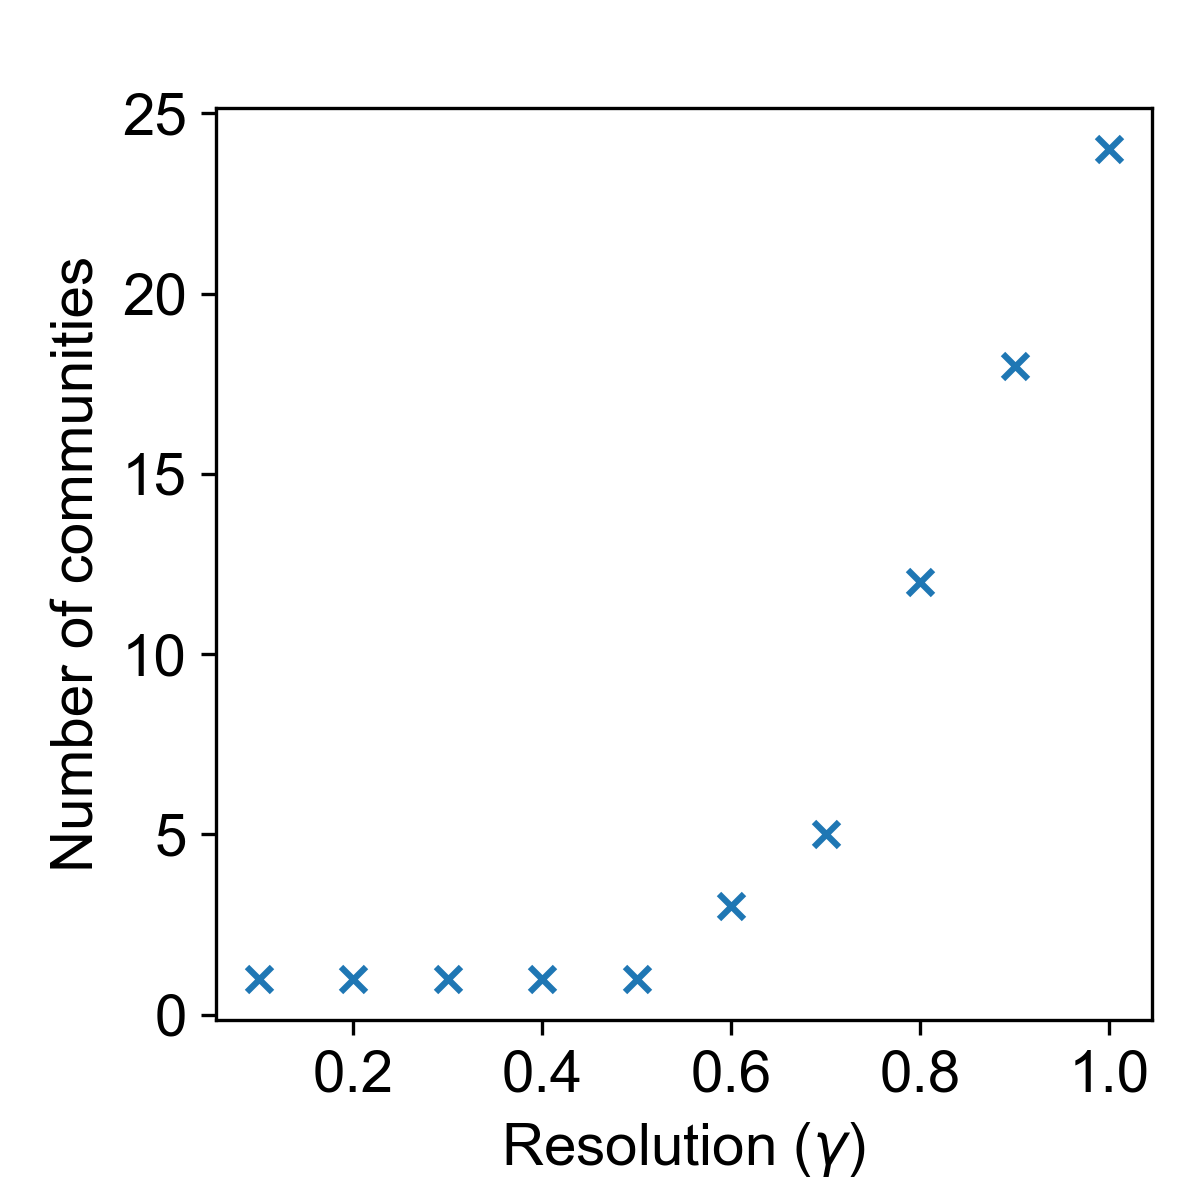
\includegraphics[keepaspectratio,width=\textwidth,height=0.375\textheight]{Random_Leiden_by_gamma.png}
\caption[]{Decreasing the resolution parameter $\gamma$ results in lower number of communities also in the random graph generated from PBMC 3k data. At $\gamma < 0.5$, Leiden approach correctly identifies one single community.}
\label{Modularity_Random_Res}
\end{figure}
\clearpage


%\begin{figure}[htbp]
%\centering
%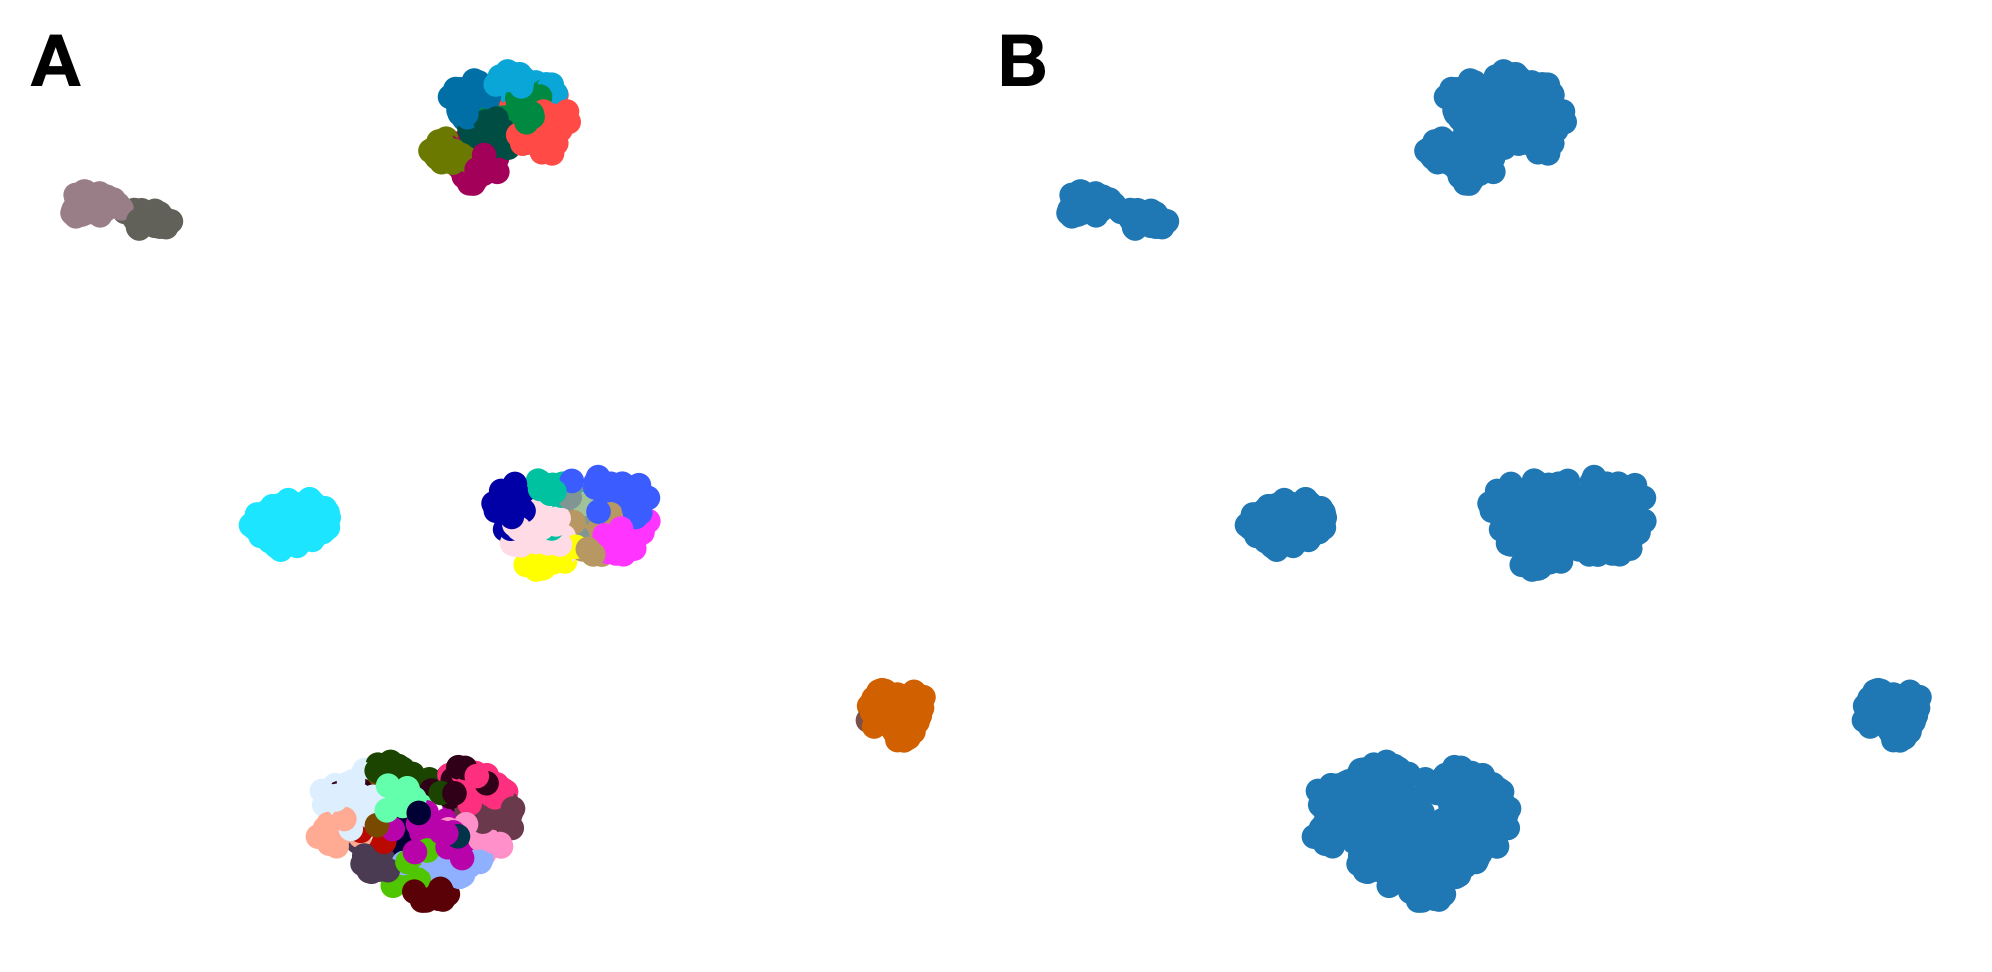
\includegraphics[keepaspectratio,width=\textwidth,height=0.75\textheight]{Tian_NSBM0.png}
%\caption[]{Analysis of a mixture of 5 known cell lines. (A) UMAP  embedding of cell lines from the sc-mixology experiment coloured by the level 0 of the hierarchy proposed by the nested Stochastic Block Model (B) UMAP embedding coloured by the classification made by SCCAF when partitions in (A) are used.}\label{Tian_NSBM0}
%\end{figure}
%\clearpage
%\begin{figure}[htbp]
%\centering
%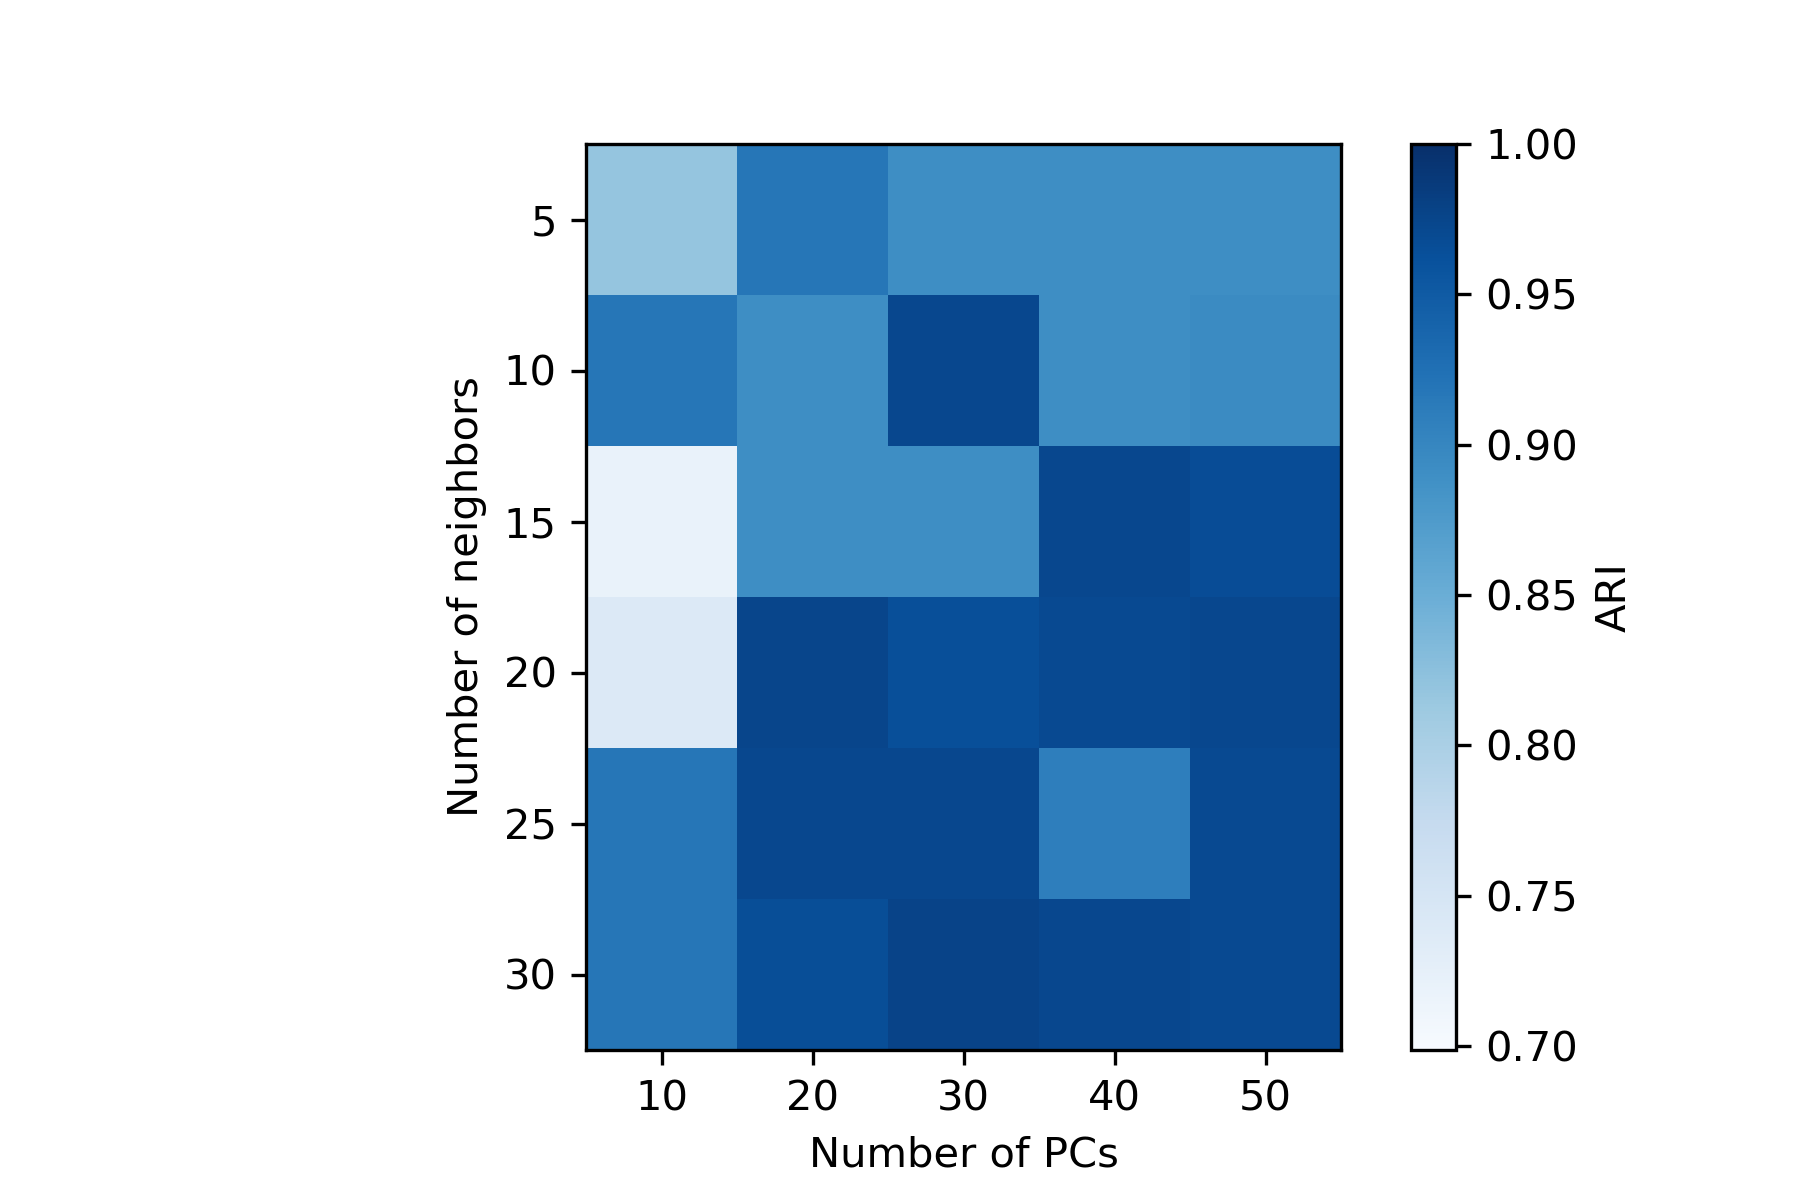
\includegraphics[keepaspectratio,width=\textwidth,height=0.75\textheight]{Figure_S2.png}
%\caption[]{Adjusted Rand Index for different \emph{k}NN graphs after MCMC run. Maximal ARI over all hierarchy level is shown. Darker color indicates higher concordance with the ground truth}\label{MPFigure:9060BBC5-898E-4AA7-A57D-D221167F7250}
%\end{figure}

\begin{figure}[htbp]
\centering
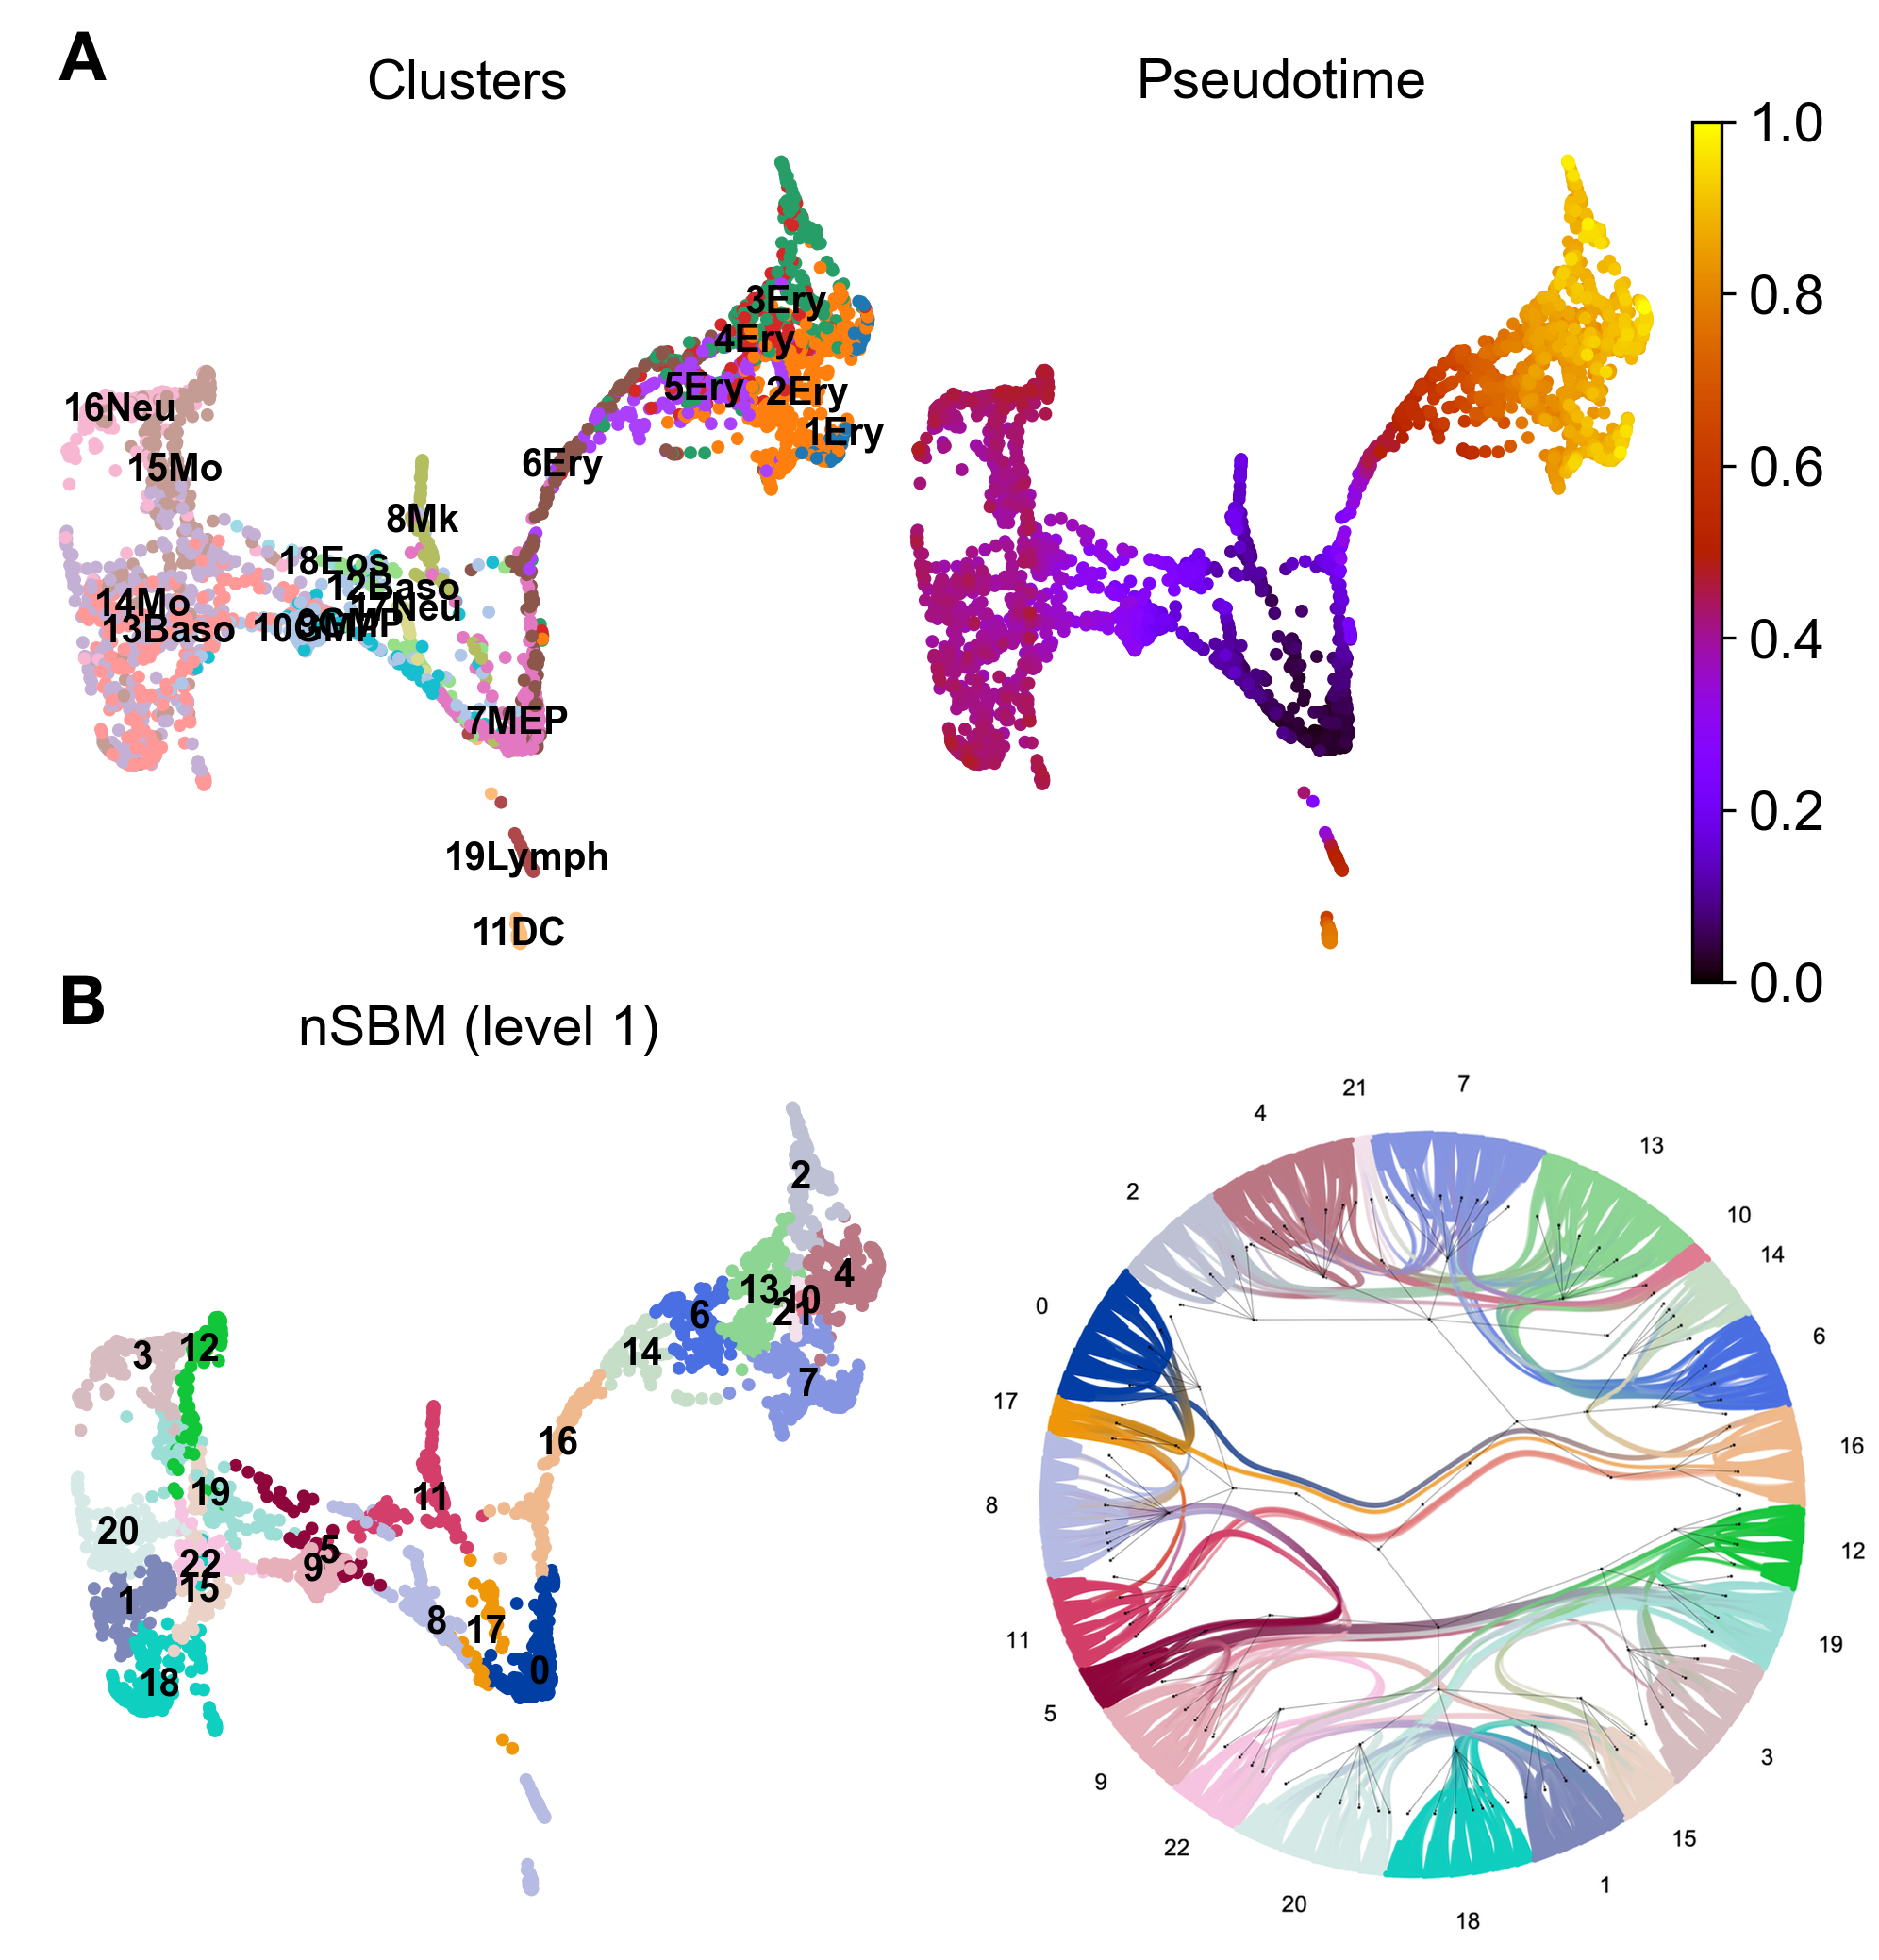
\includegraphics[keepaspectratio,width=\textwidth,height=0.75\textheight]{Figure_Hemato_Supp.pdf}
\caption[]{Low dimensional embedding of single cells from hematopoietic differentiation dataset. Cells are colored by original cell type (A), pseudotime (B), nSBM grouping at level \textcolor{red}{1} of the hierarchy (C) and level 0 (D). Since level 0 identifies 114 groups, only group labels have been represented.}\label{Figure_Hemato_Supp}
\end{figure}
\clearpage

\begin{figure}[htbp]
\centering
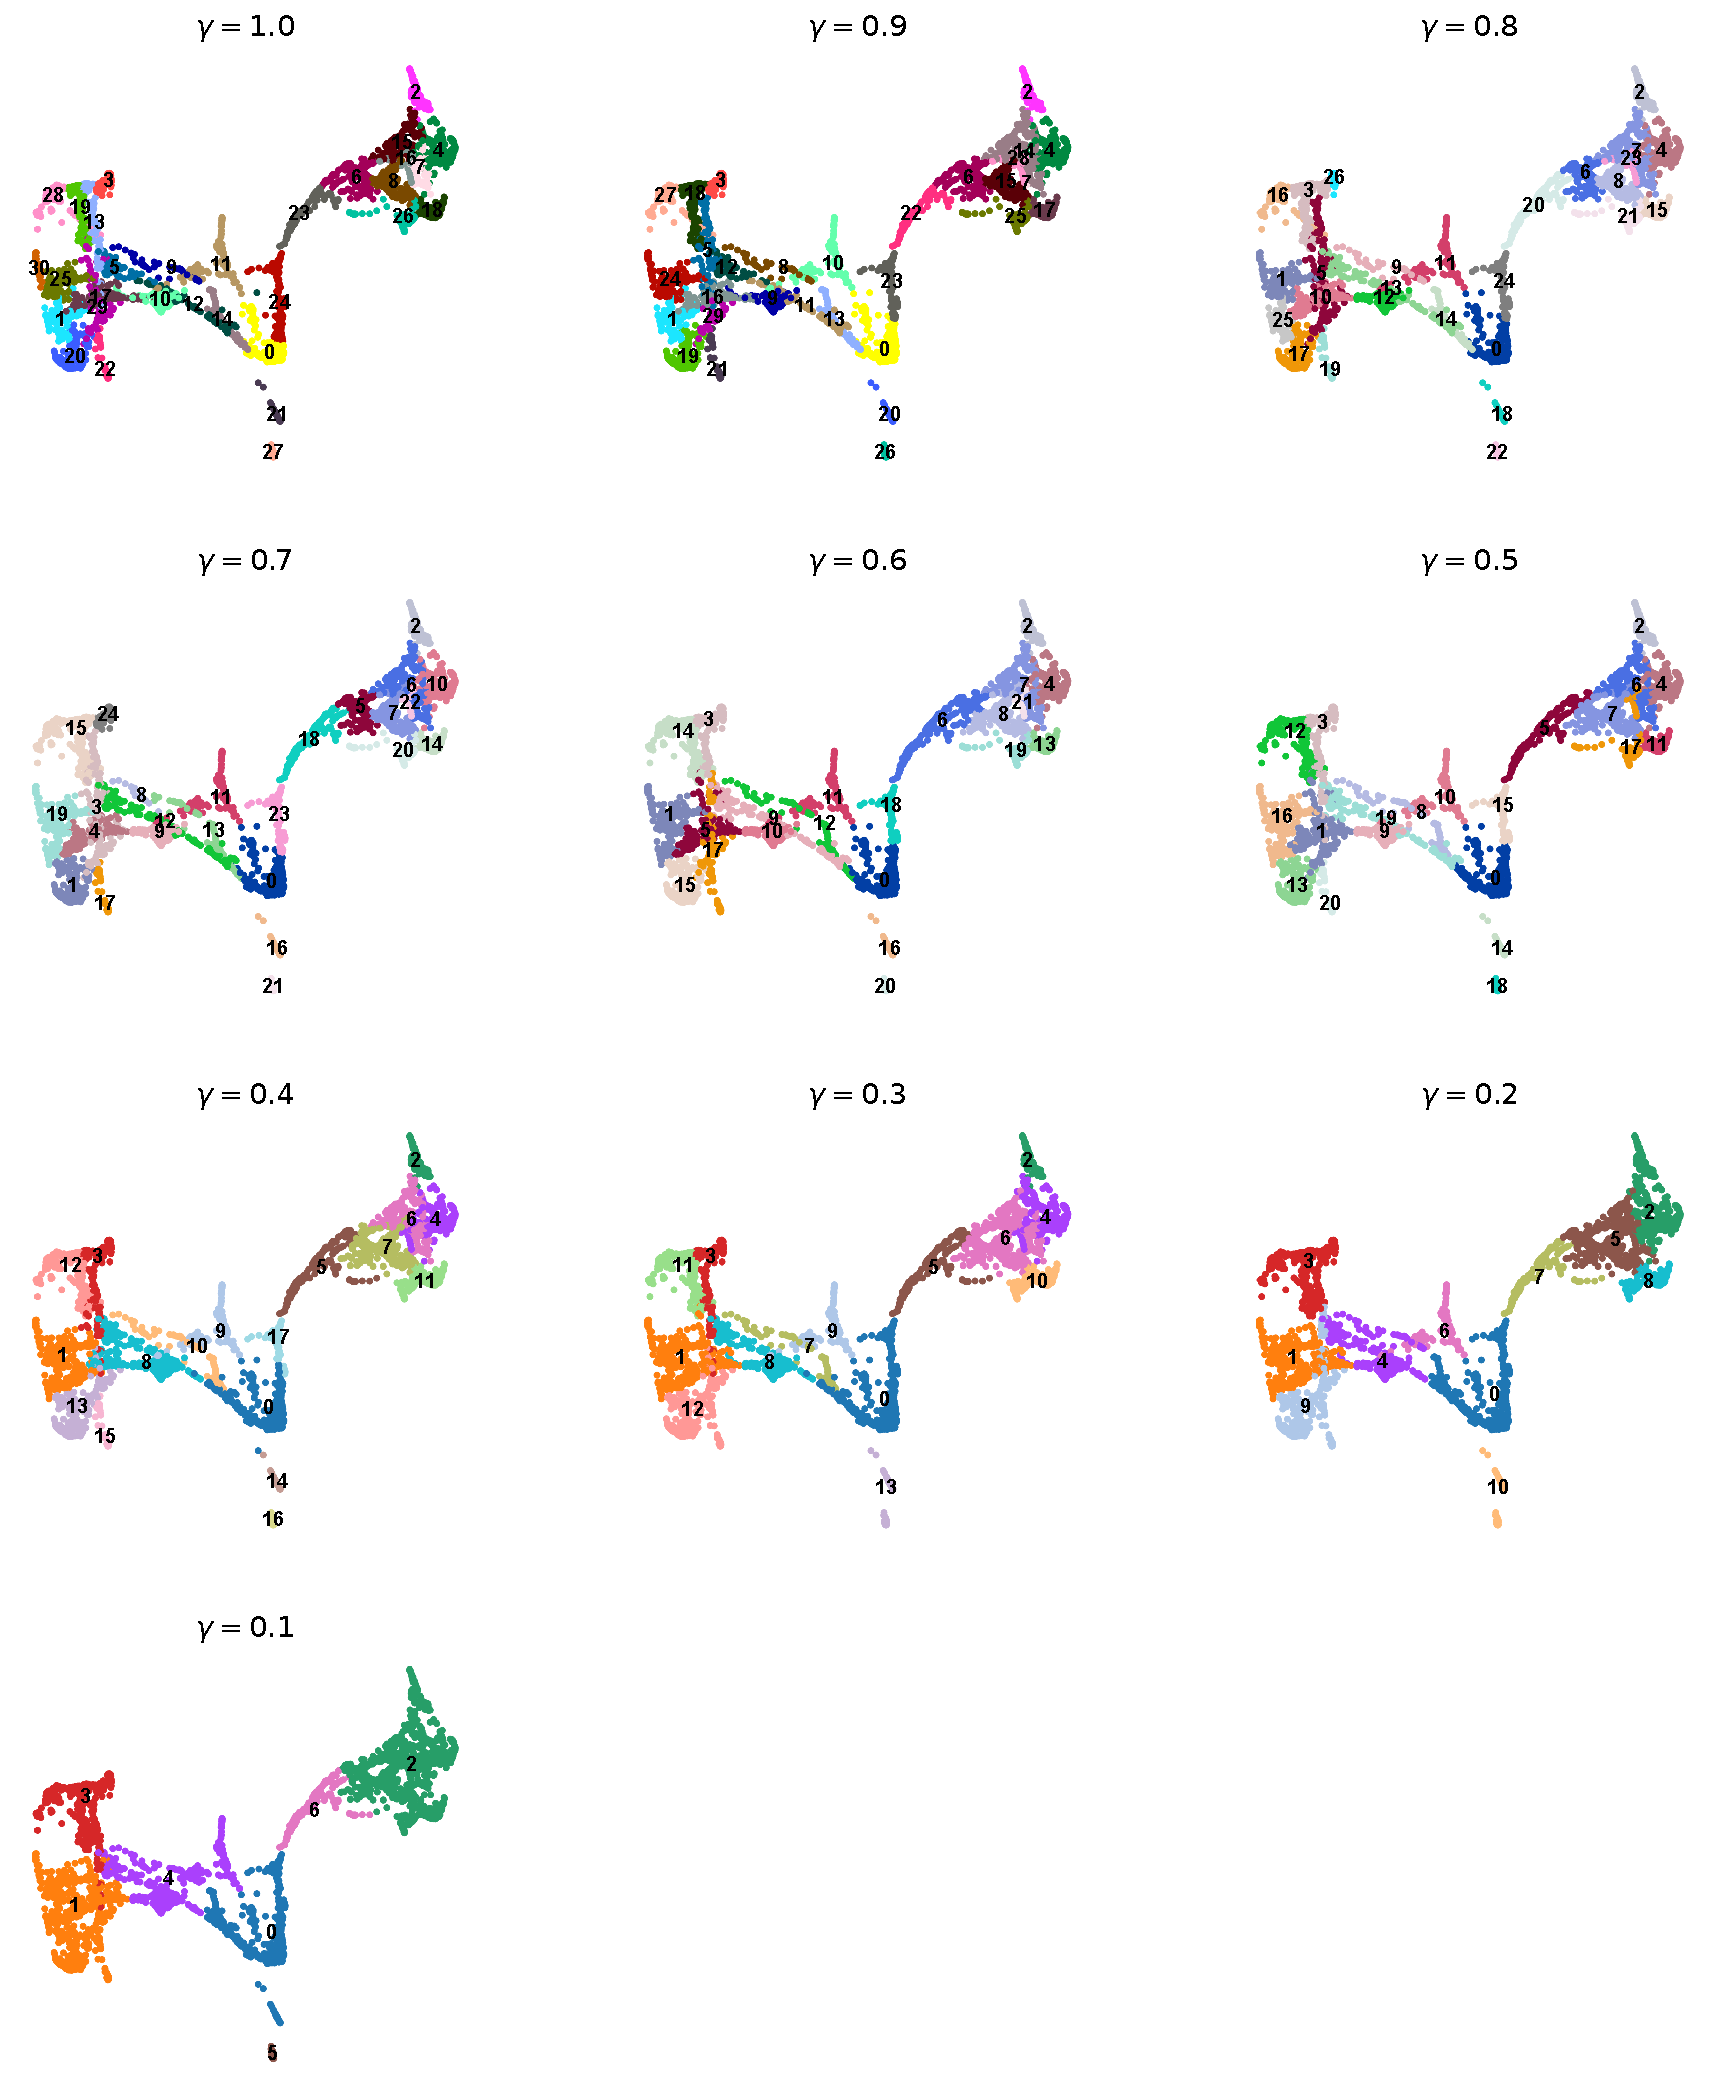
\includegraphics[keepaspectratio,width=\textwidth,height=0.75\textheight]{Figure_Paul15_Leiden_r.pdf}
\caption[]{Low dimension embedding of single cells for hematopoietic differentiation coloured according to Leiden clustering at decreasing resolution, from 1.0 to 0.1. Lowering the distribution does not grant that cells are grouped in a hierarchical way, \emph{e.g.} groups 6 and 8 in the Erythroid branch at resolution $\gamma=1$ are merged or split at coarser resolutions ($\gamma=0.6$ and $\gamma=0.3$).}\label{Figure_Paul15_Leiden_r}
\end{figure}
\clearpage

\begin{figure}[htbp]
\centering
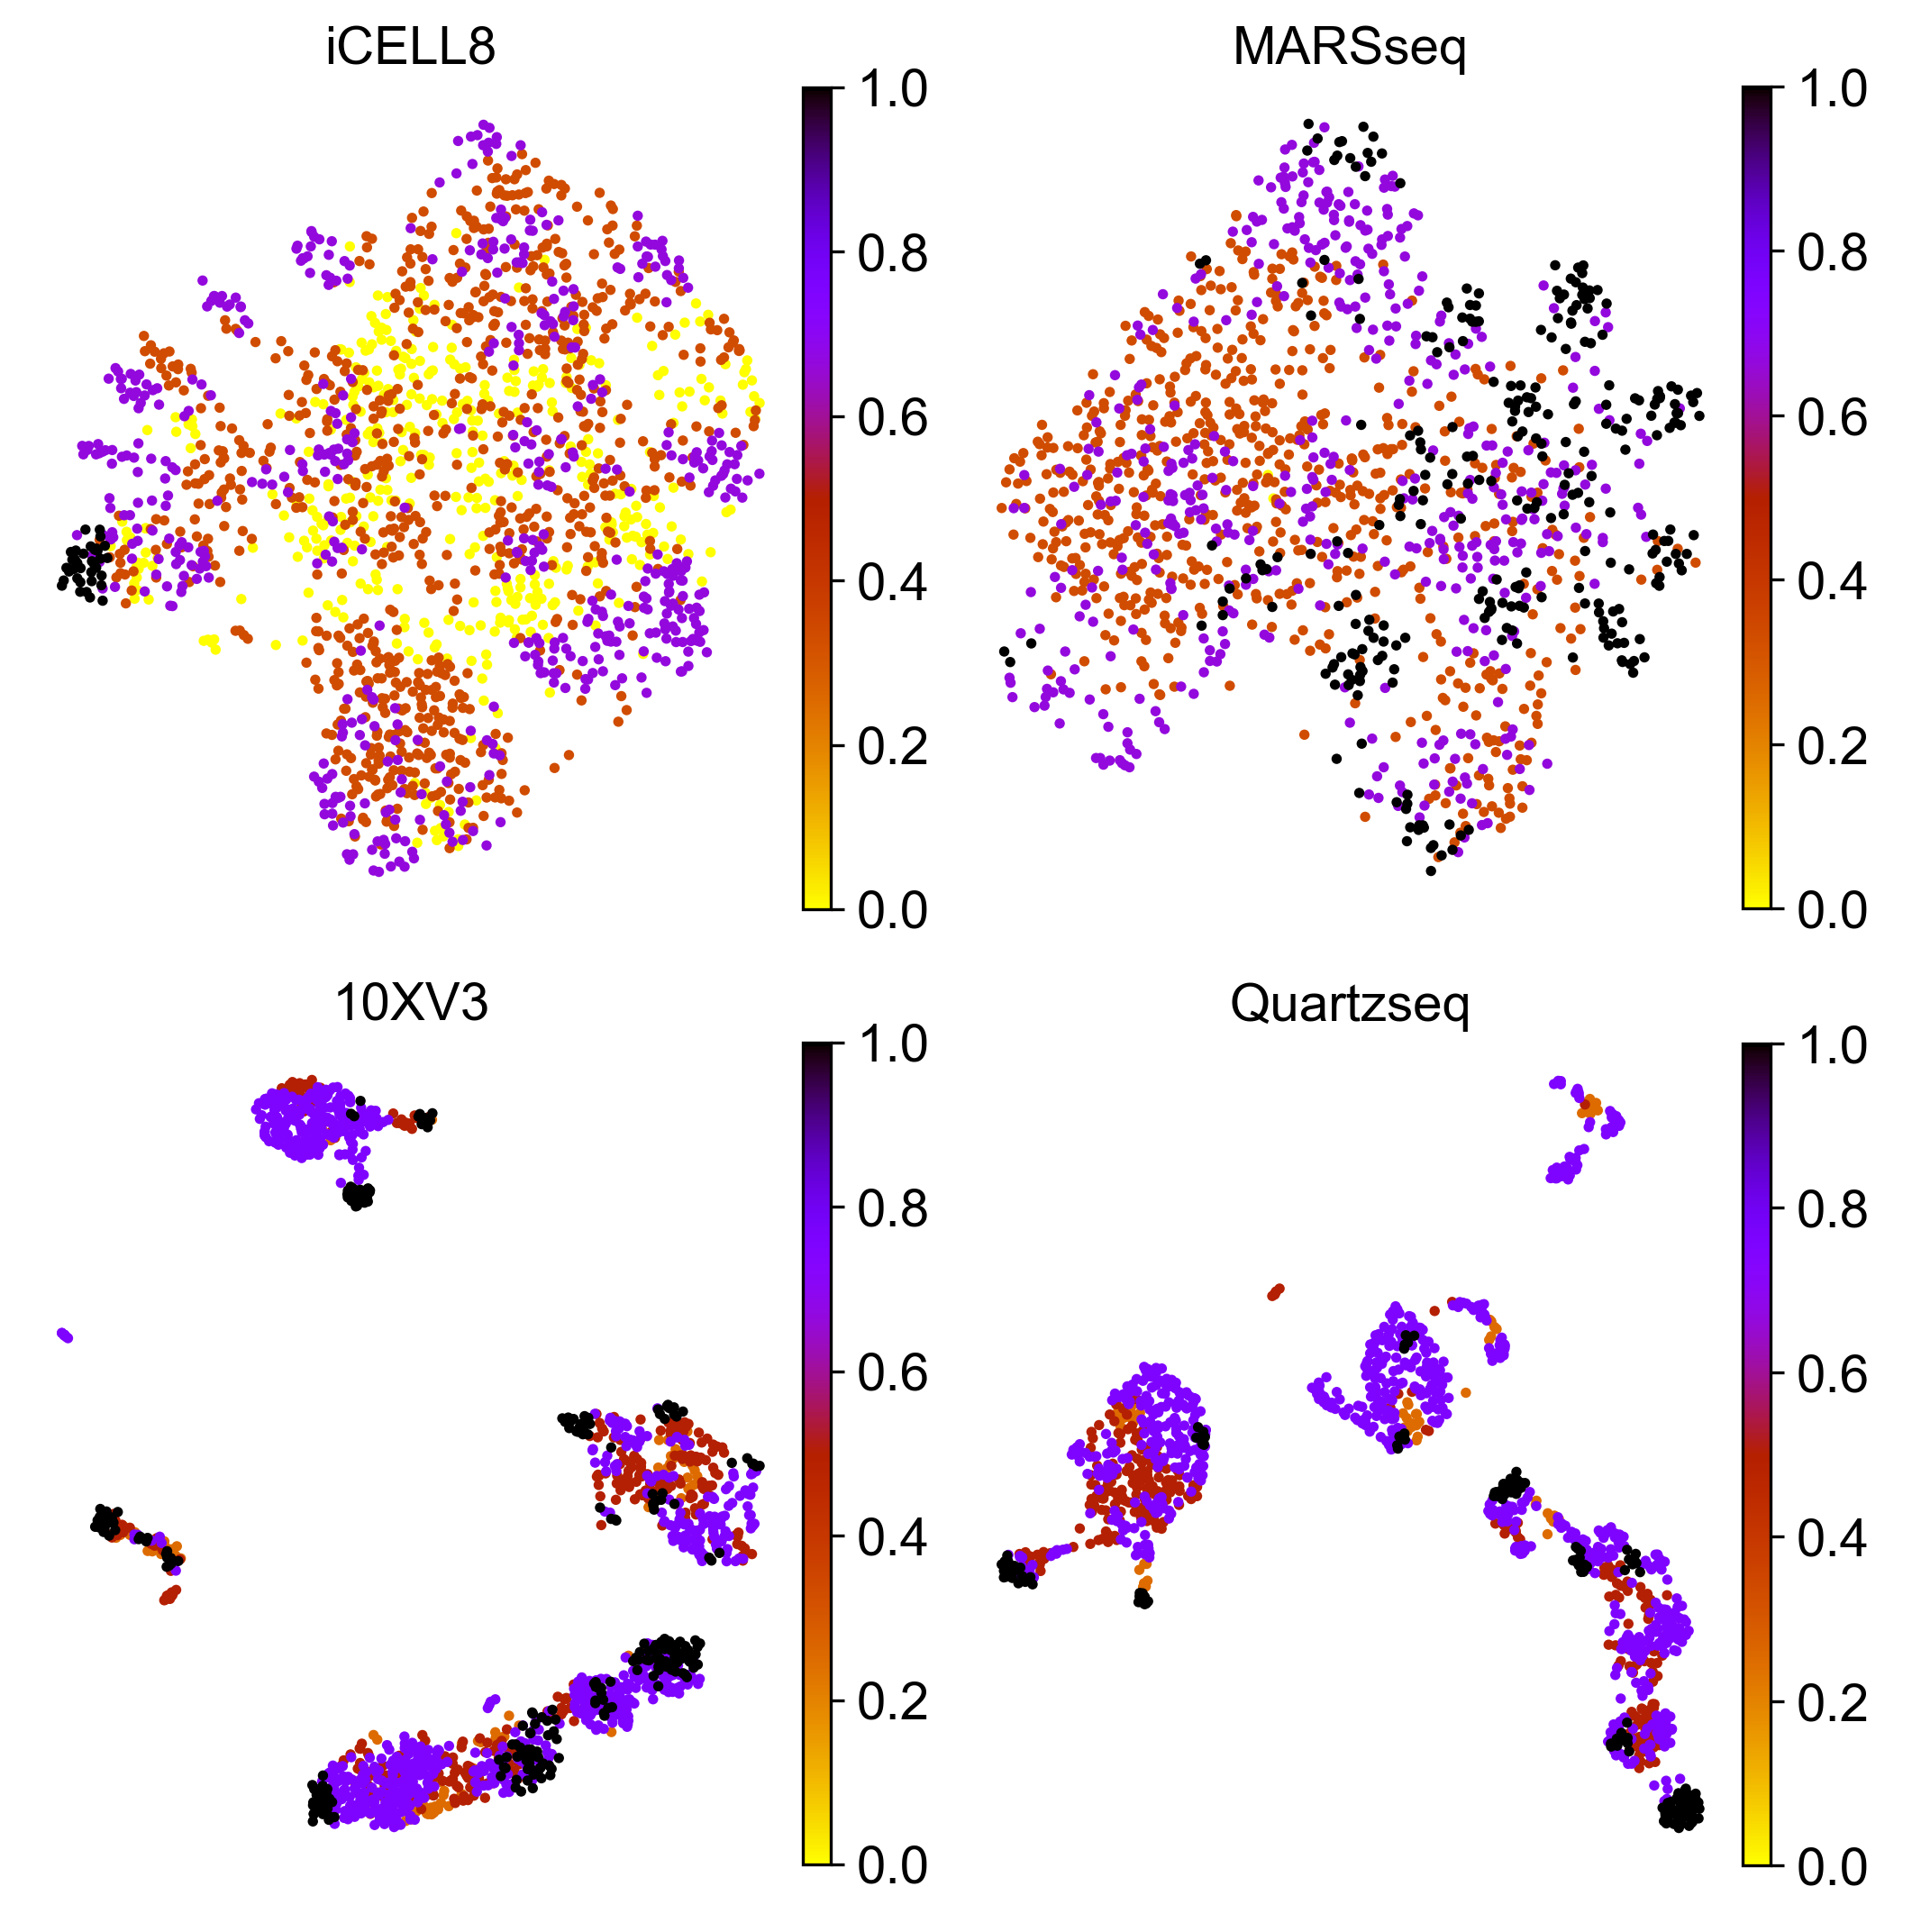
\includegraphics[keepaspectratio,width=\textwidth,width=0.50\textheight]{Figure_Stability.png}
\caption[]{Cell Stability. UMAP embeddings of PBMC data profiled with four different technologies ranked by their quality. Cells are coloured by the Cell Stability metric.}\label{Figure_Stability}
\end{figure}
\clearpage

%\begin{figure}[htbp]
%\centering
%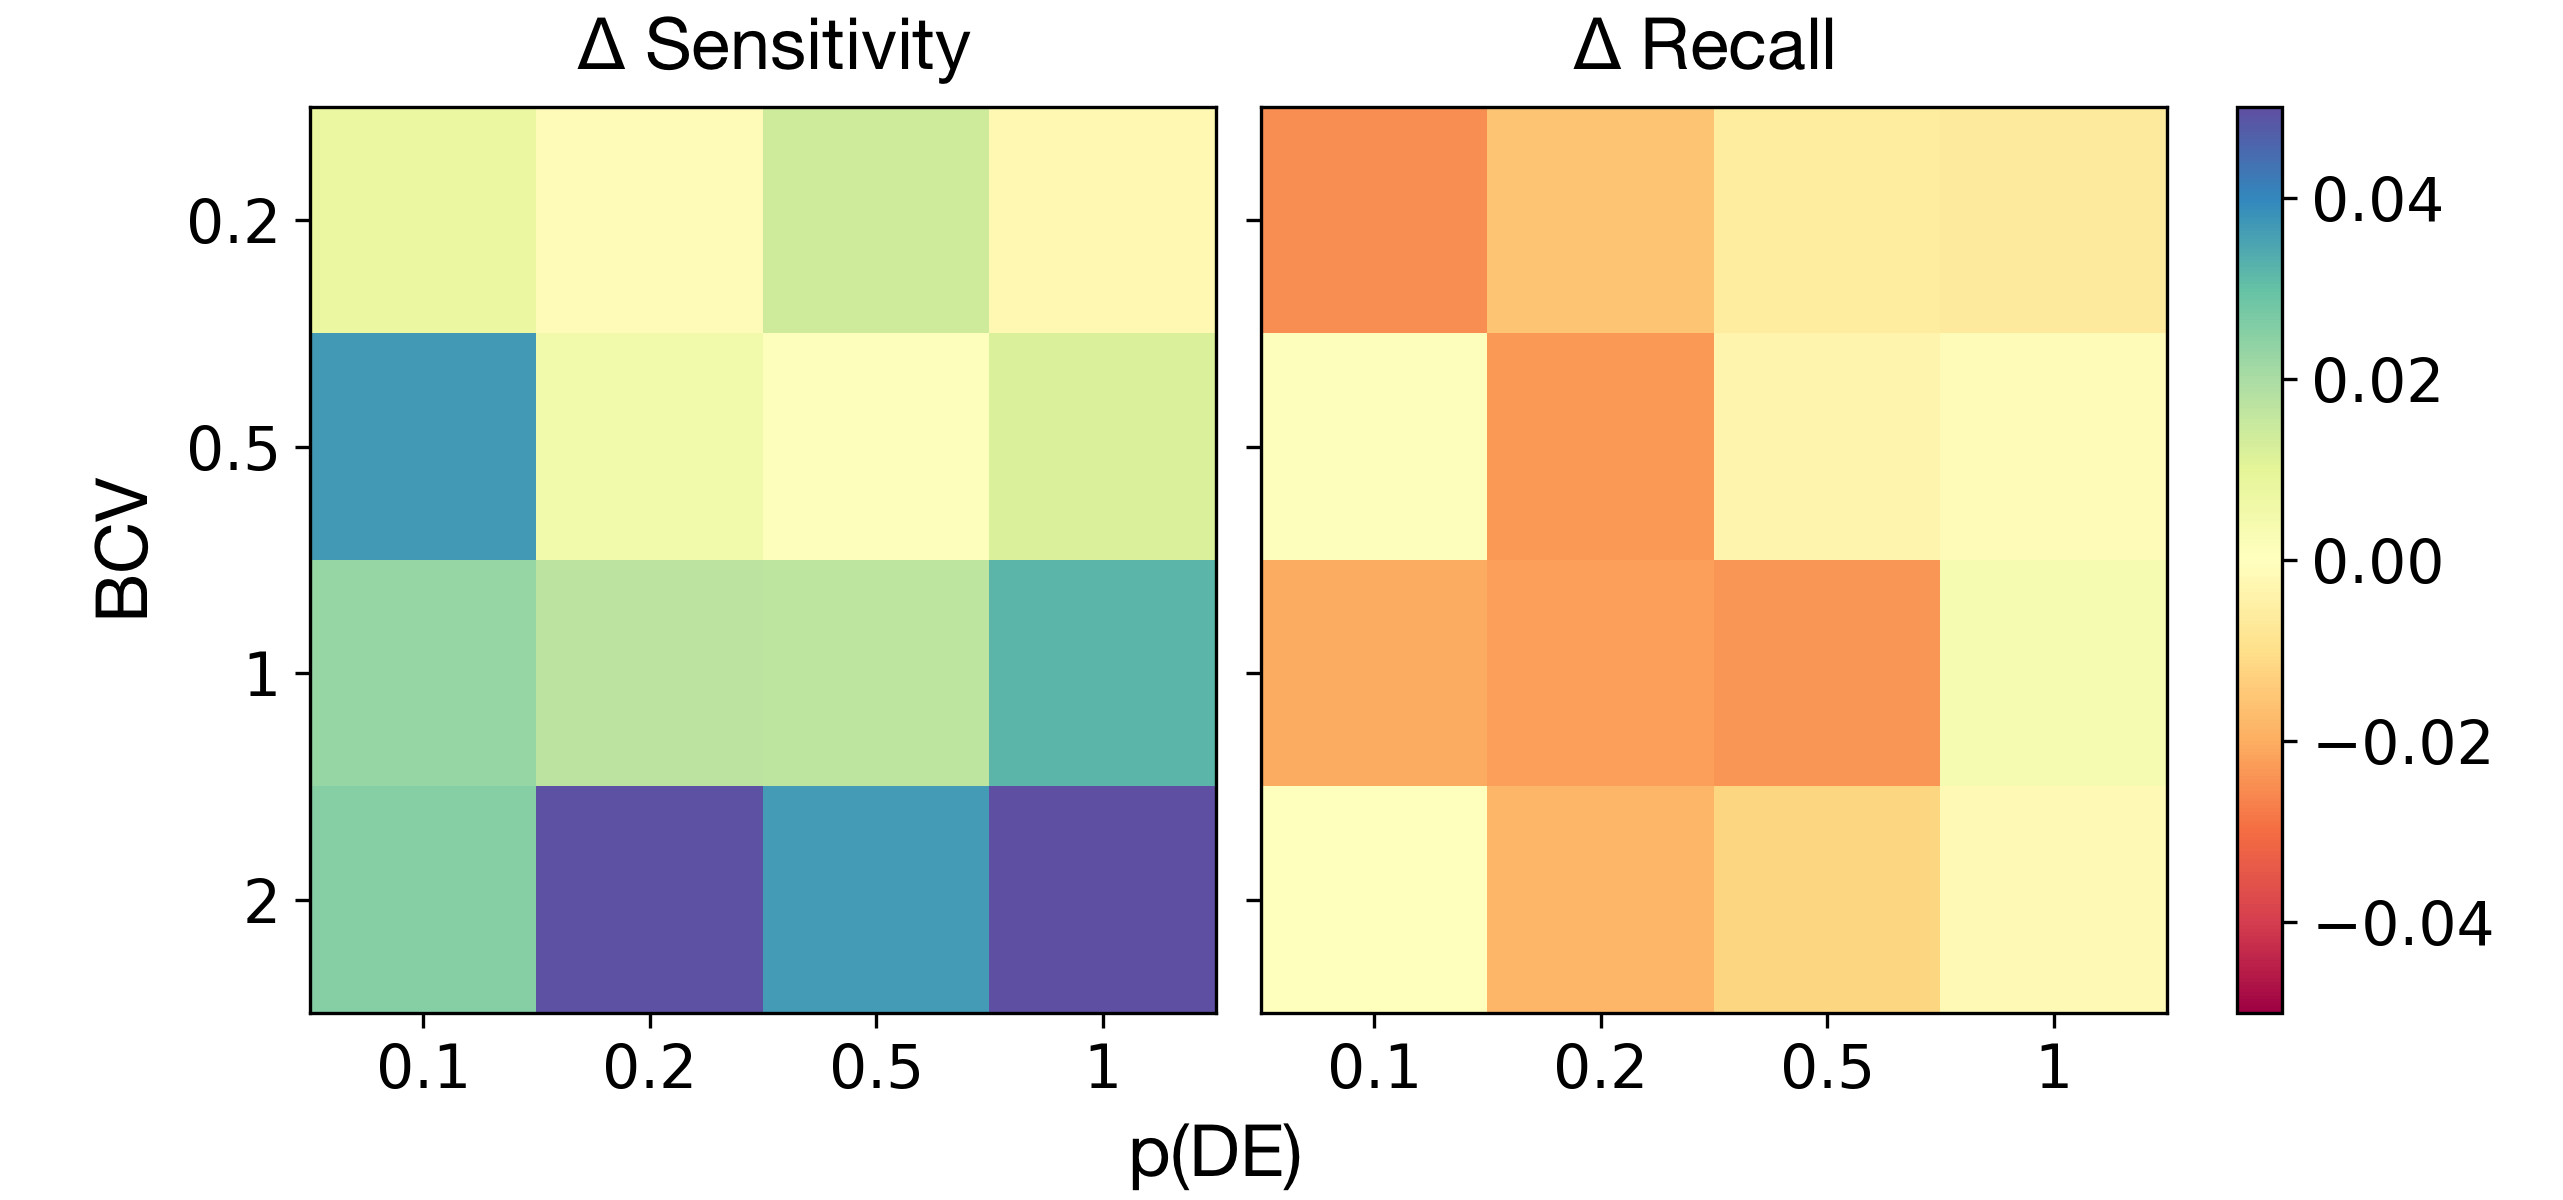
\includegraphics[keepaspectratio,width=\textwidth,width=0.50\textheight]{Figure_DE.png}
%\caption[]{Results of differential gene expression with or without marginals. The heatmaps show the difference in sensitivity (left) or recall (right) of statistical testing for differential genes among cell groups when marginals are included or not in the model. Tests have been conducted on simulated data with different levels of noise (BCV) or probability of differential expression (p(DE))}\label{Figure_DE}
%\end{figure}
%\clearpage


\begin{figure}[htbp]
\centering
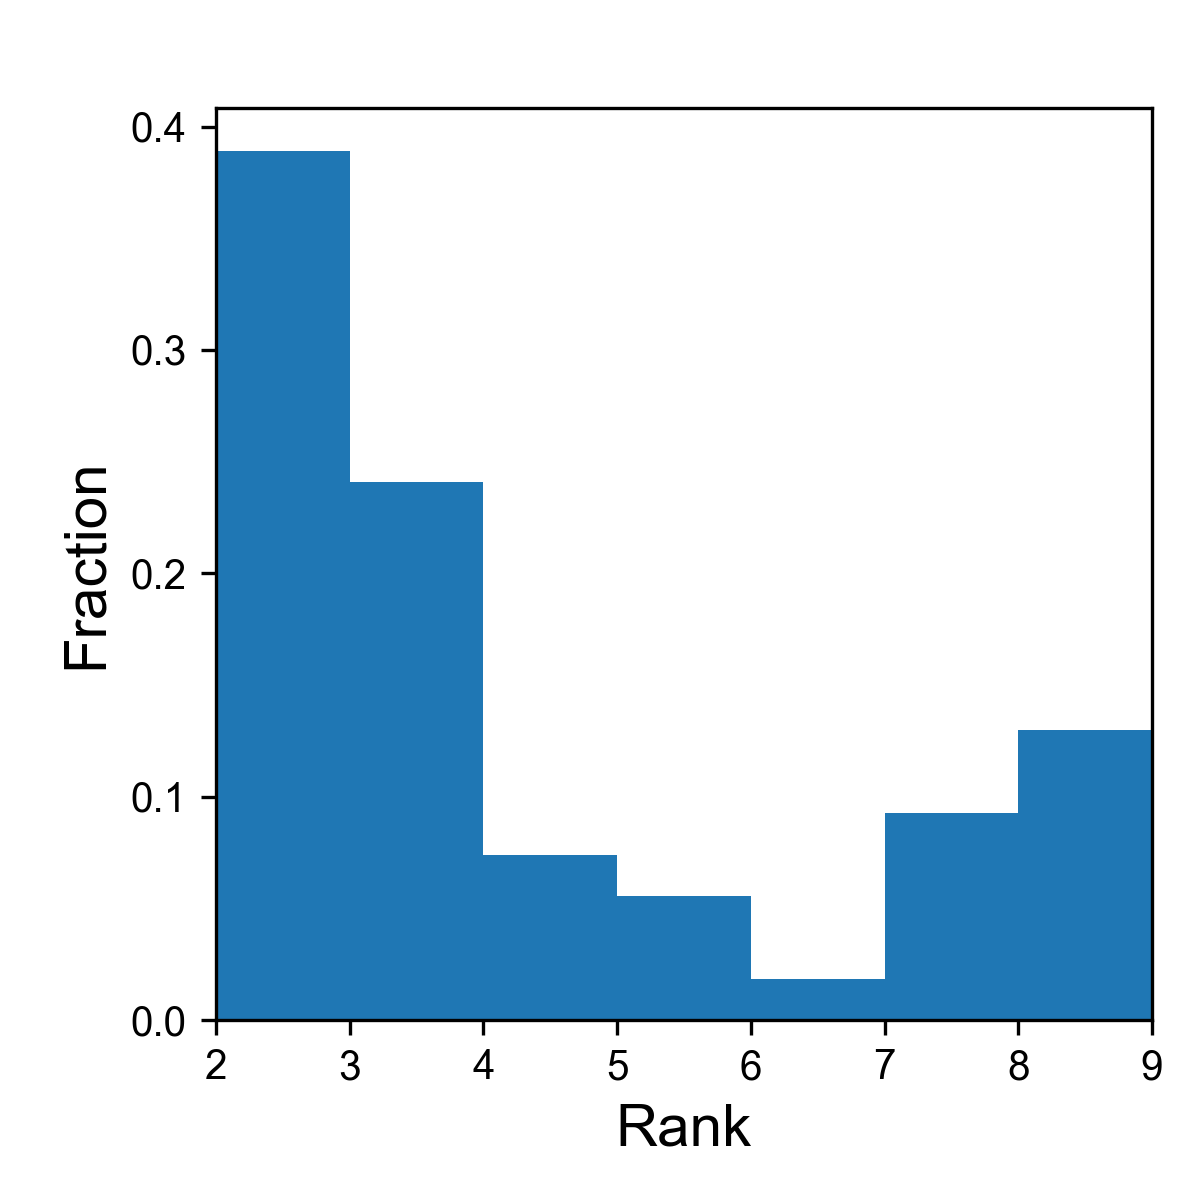
\includegraphics[keepaspectratio,width=\textwidth,height=0.75\textheight]{hist_label_second.png}
\caption[]{Distribution of second choices in label transfer. For each dataset in which we assessed accuracy of label transfer by SBM, we collect the rank of affinities of the correct class when an assignment could not be performed (\emph{i.e.} the highest affinity was for the "Unknonwn" label)  }\label{hist_label_second}
\end{figure}
\clearpage

\begin{figure}[htbp]
\centering
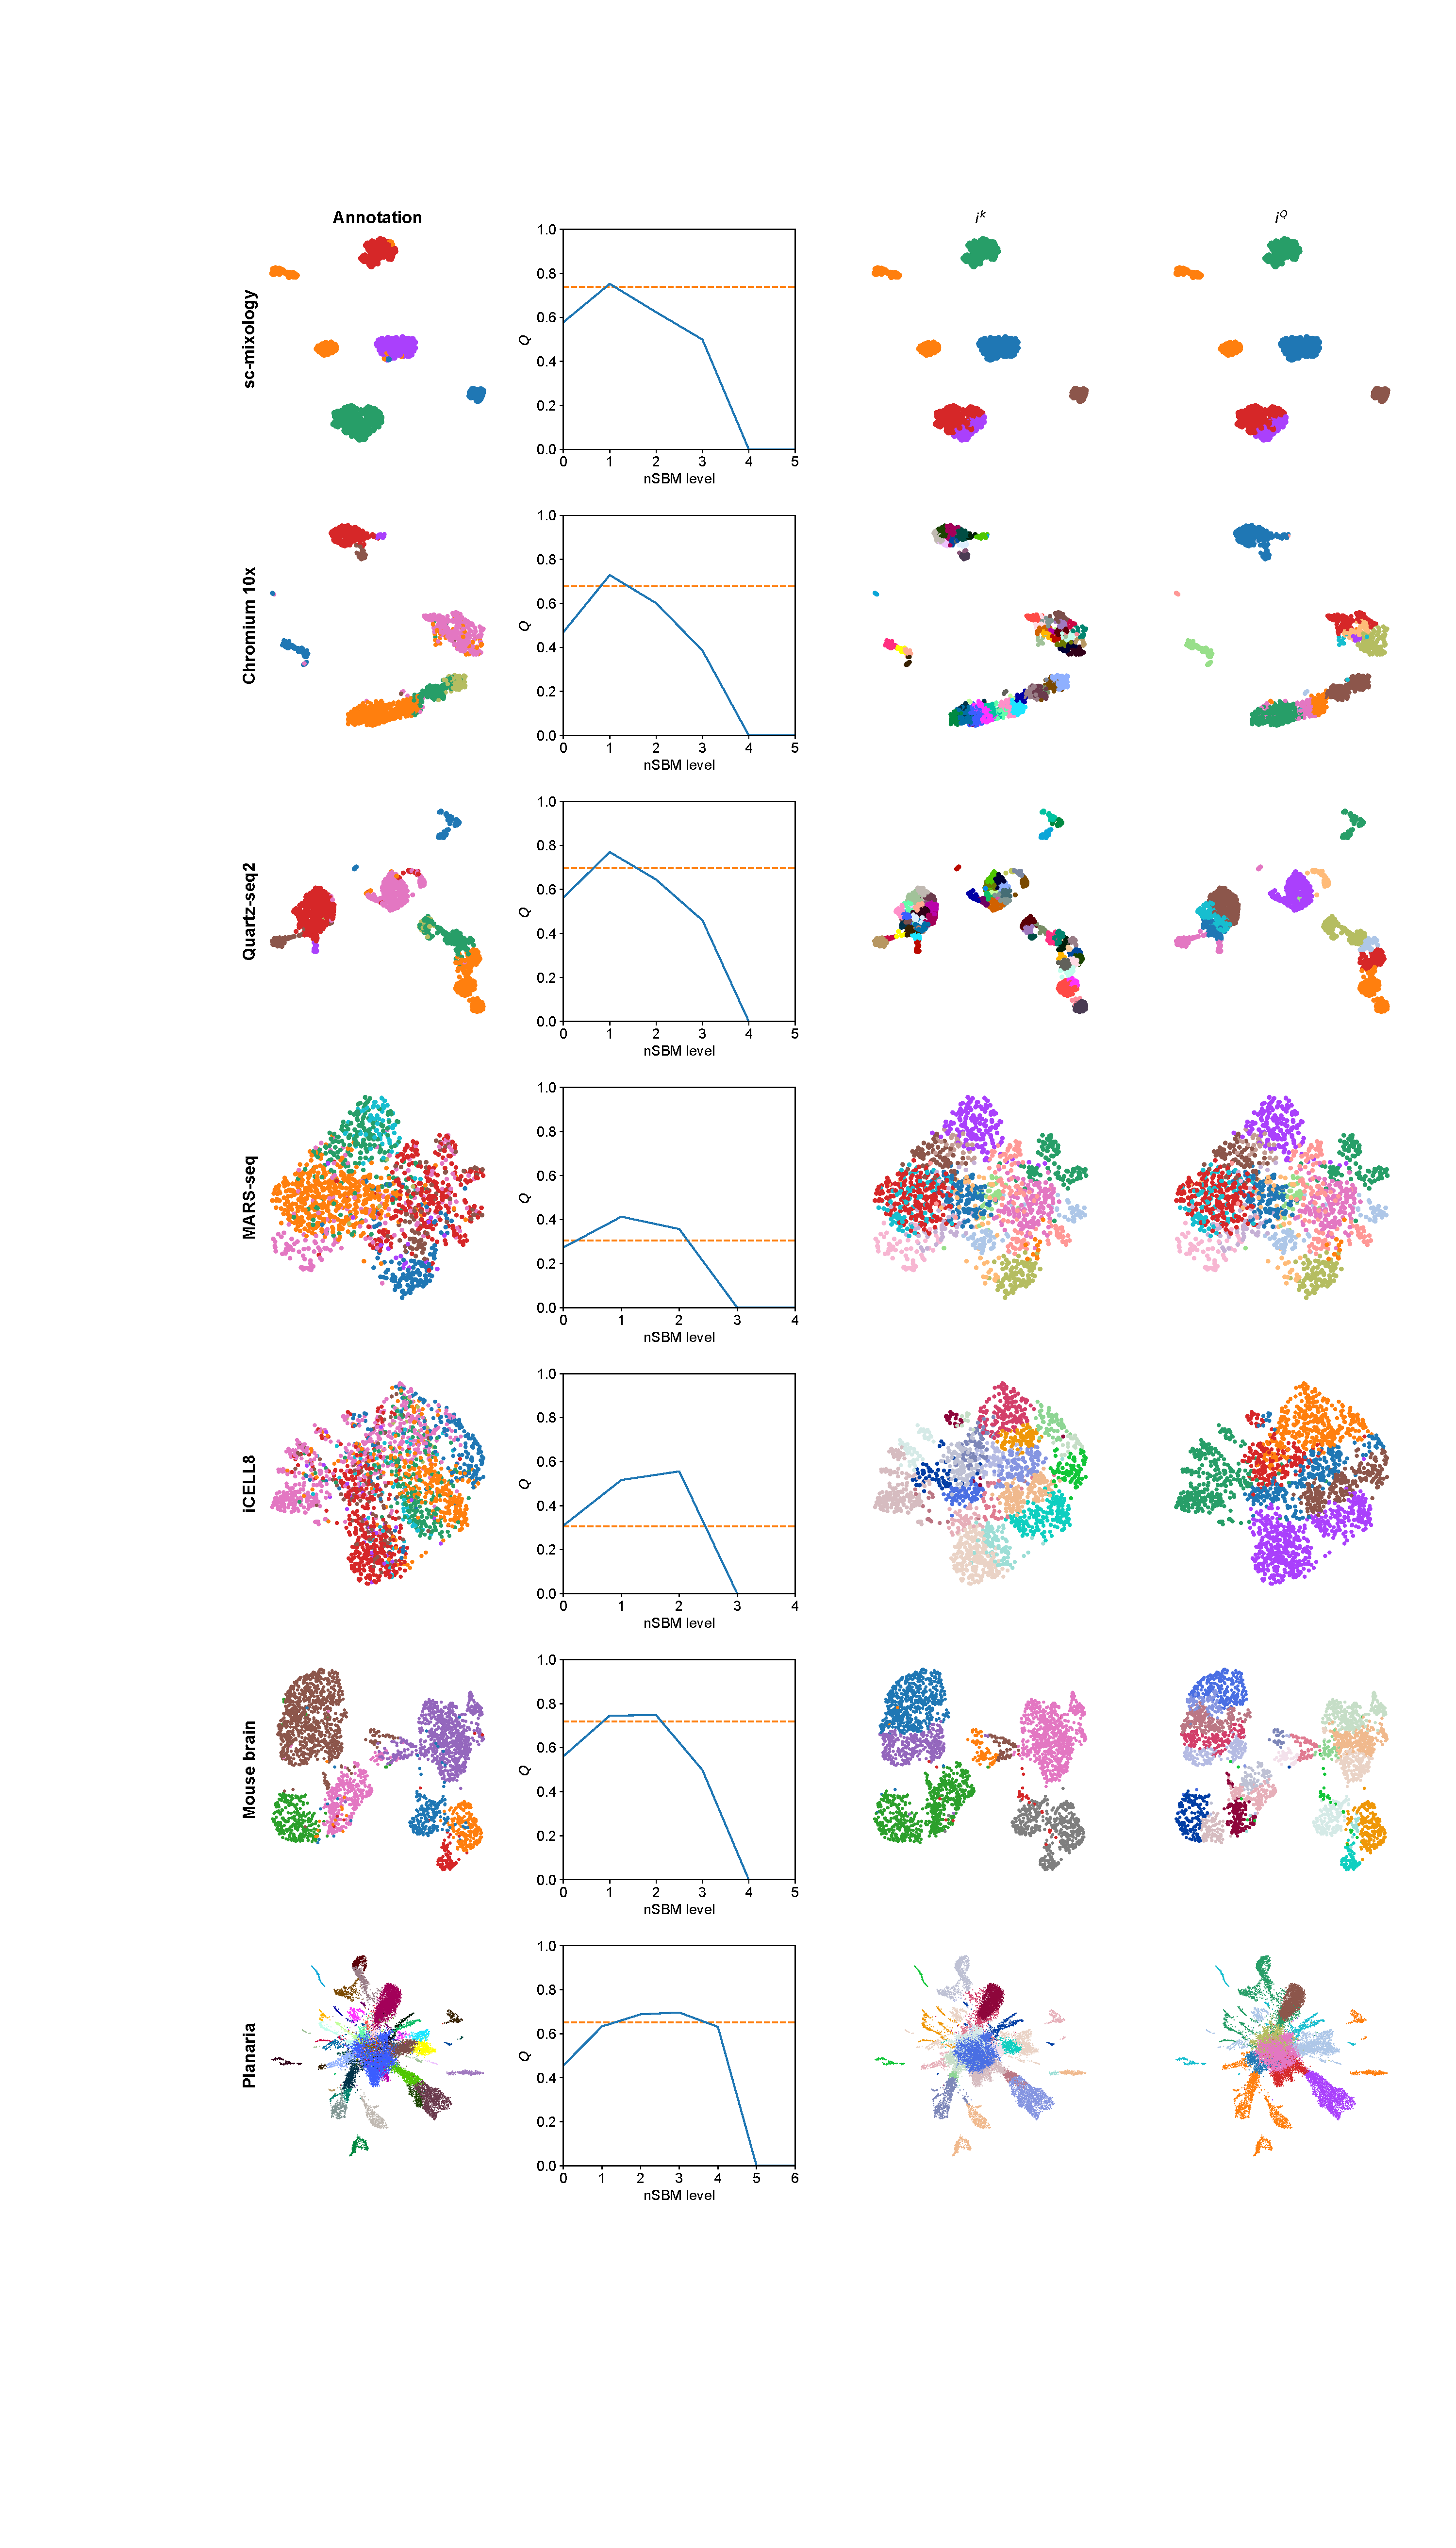
\includegraphics[keepaspectratio,width=1\textwidth,height=\textheight]{FigureOptimalLevel.pdf}
\vspace*{-80pt}
\caption[]{Choice of the optimal hierarchy level. Datasets analysed for choice of the most relevant hierarchy level are represented here, from top to bottom in the same order as in Table \ref{table_optimal}. For each dataset we report the UMAP embedding coloured by the annotation given in the corresponding manuscript, the profile of modularity $Q$ at different level of the hierarchy and the UMAP embeddings coloured by the level according to $i^k$ or $i^Q$. The dashed line in modularity plots represents the modularity calculated using the annotation from the corresponding manuscripts.}\label{FigureOptimalLevel}
\end{figure}

\clearpage
\begin{figure}[H]
\centering
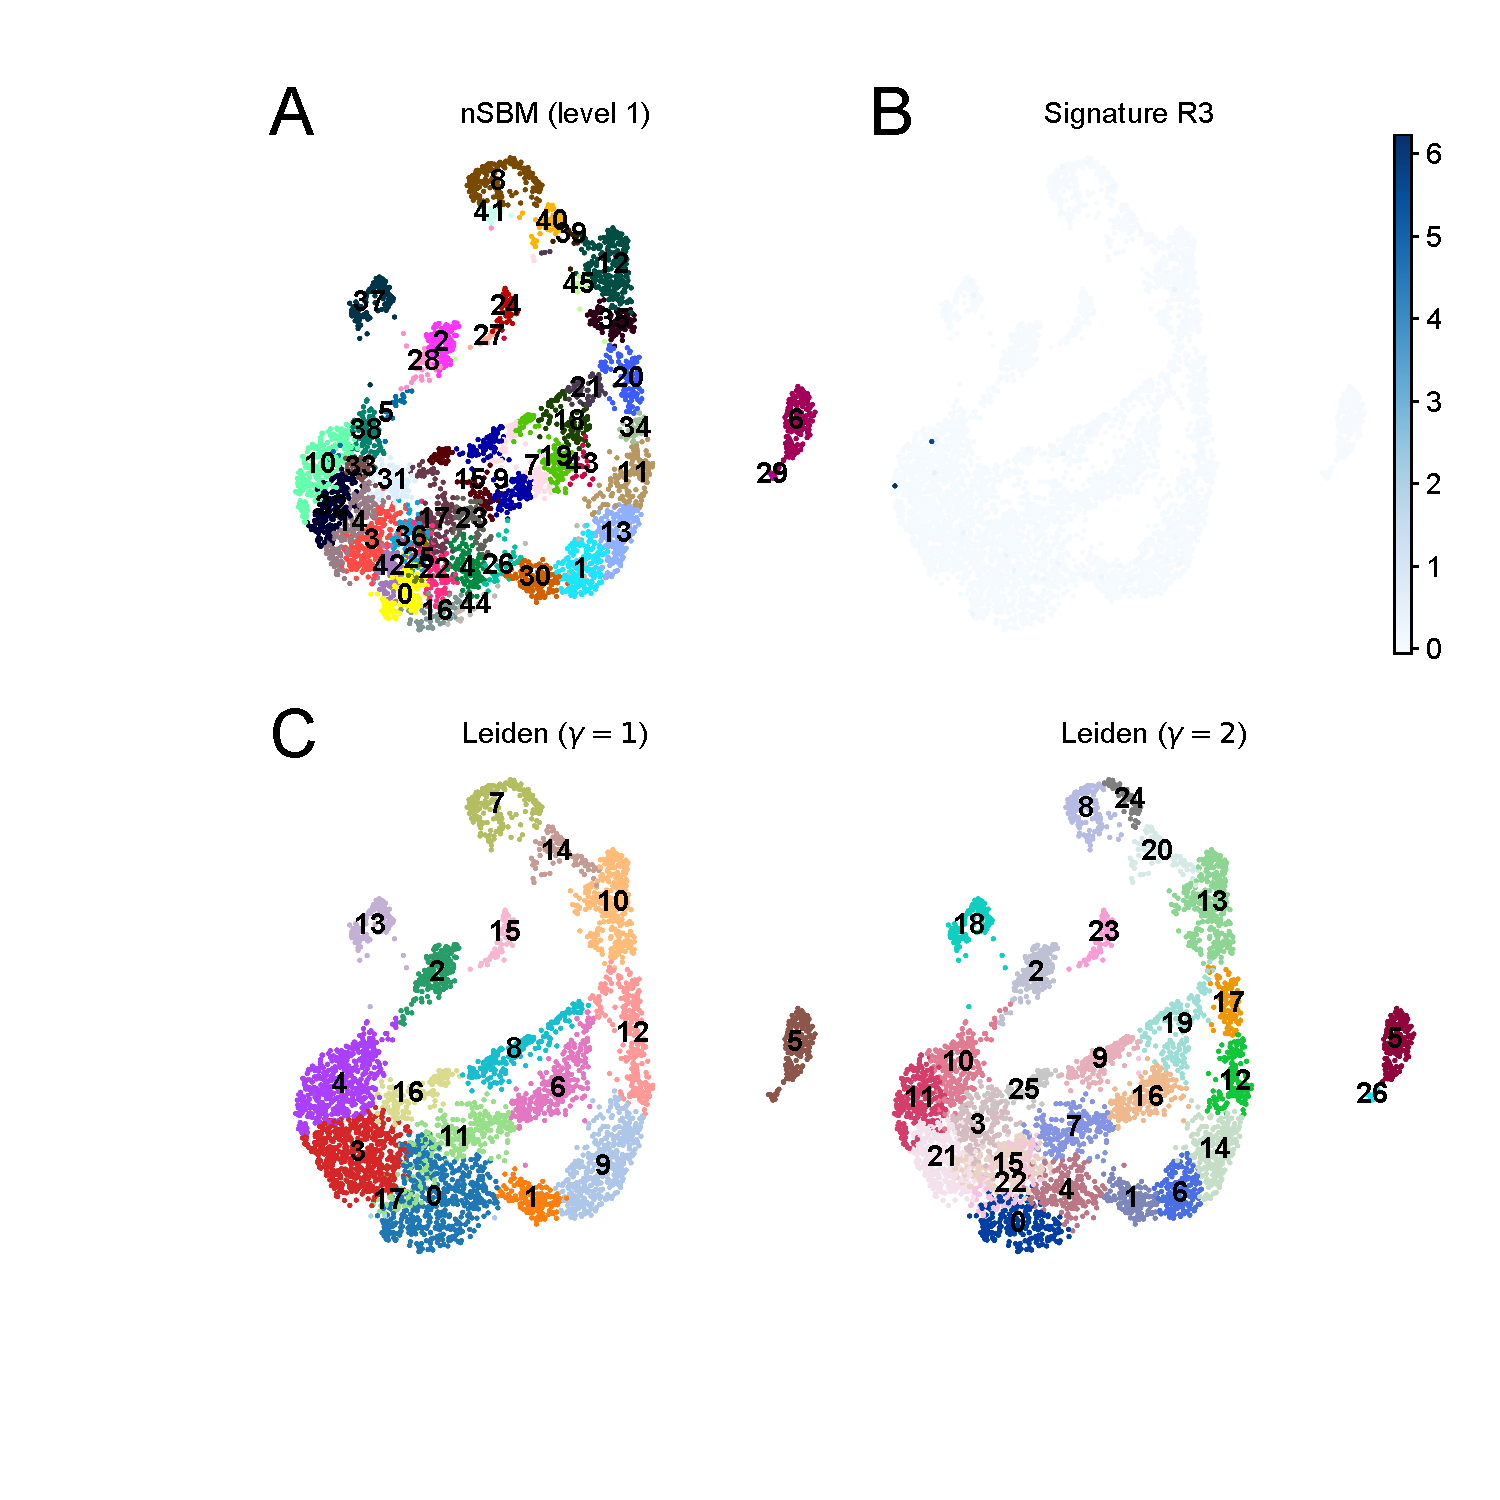
\includegraphics[keepaspectratio,width=1\textwidth,height=\textheight]{Figure_Rare_Cells_Supp.pdf}
%\vspace*{-40pt}
\caption[]{Identification of rare populations. (A) UMAP embedding of mouse crypt cells coloured by cell groups resulting at level 1 of the nSBM hierarchy. (B) Cells coloured by the signature of R3 group identified by GapClust. (C) UMAP embedding of mouse crypt cells coloured after optimisation of modularity at default parameters (left) or higher resolution (right).} \label{Figure_Rare_Supp}
\end{figure}

\clearpage
\begin{figure}[H]
\centering
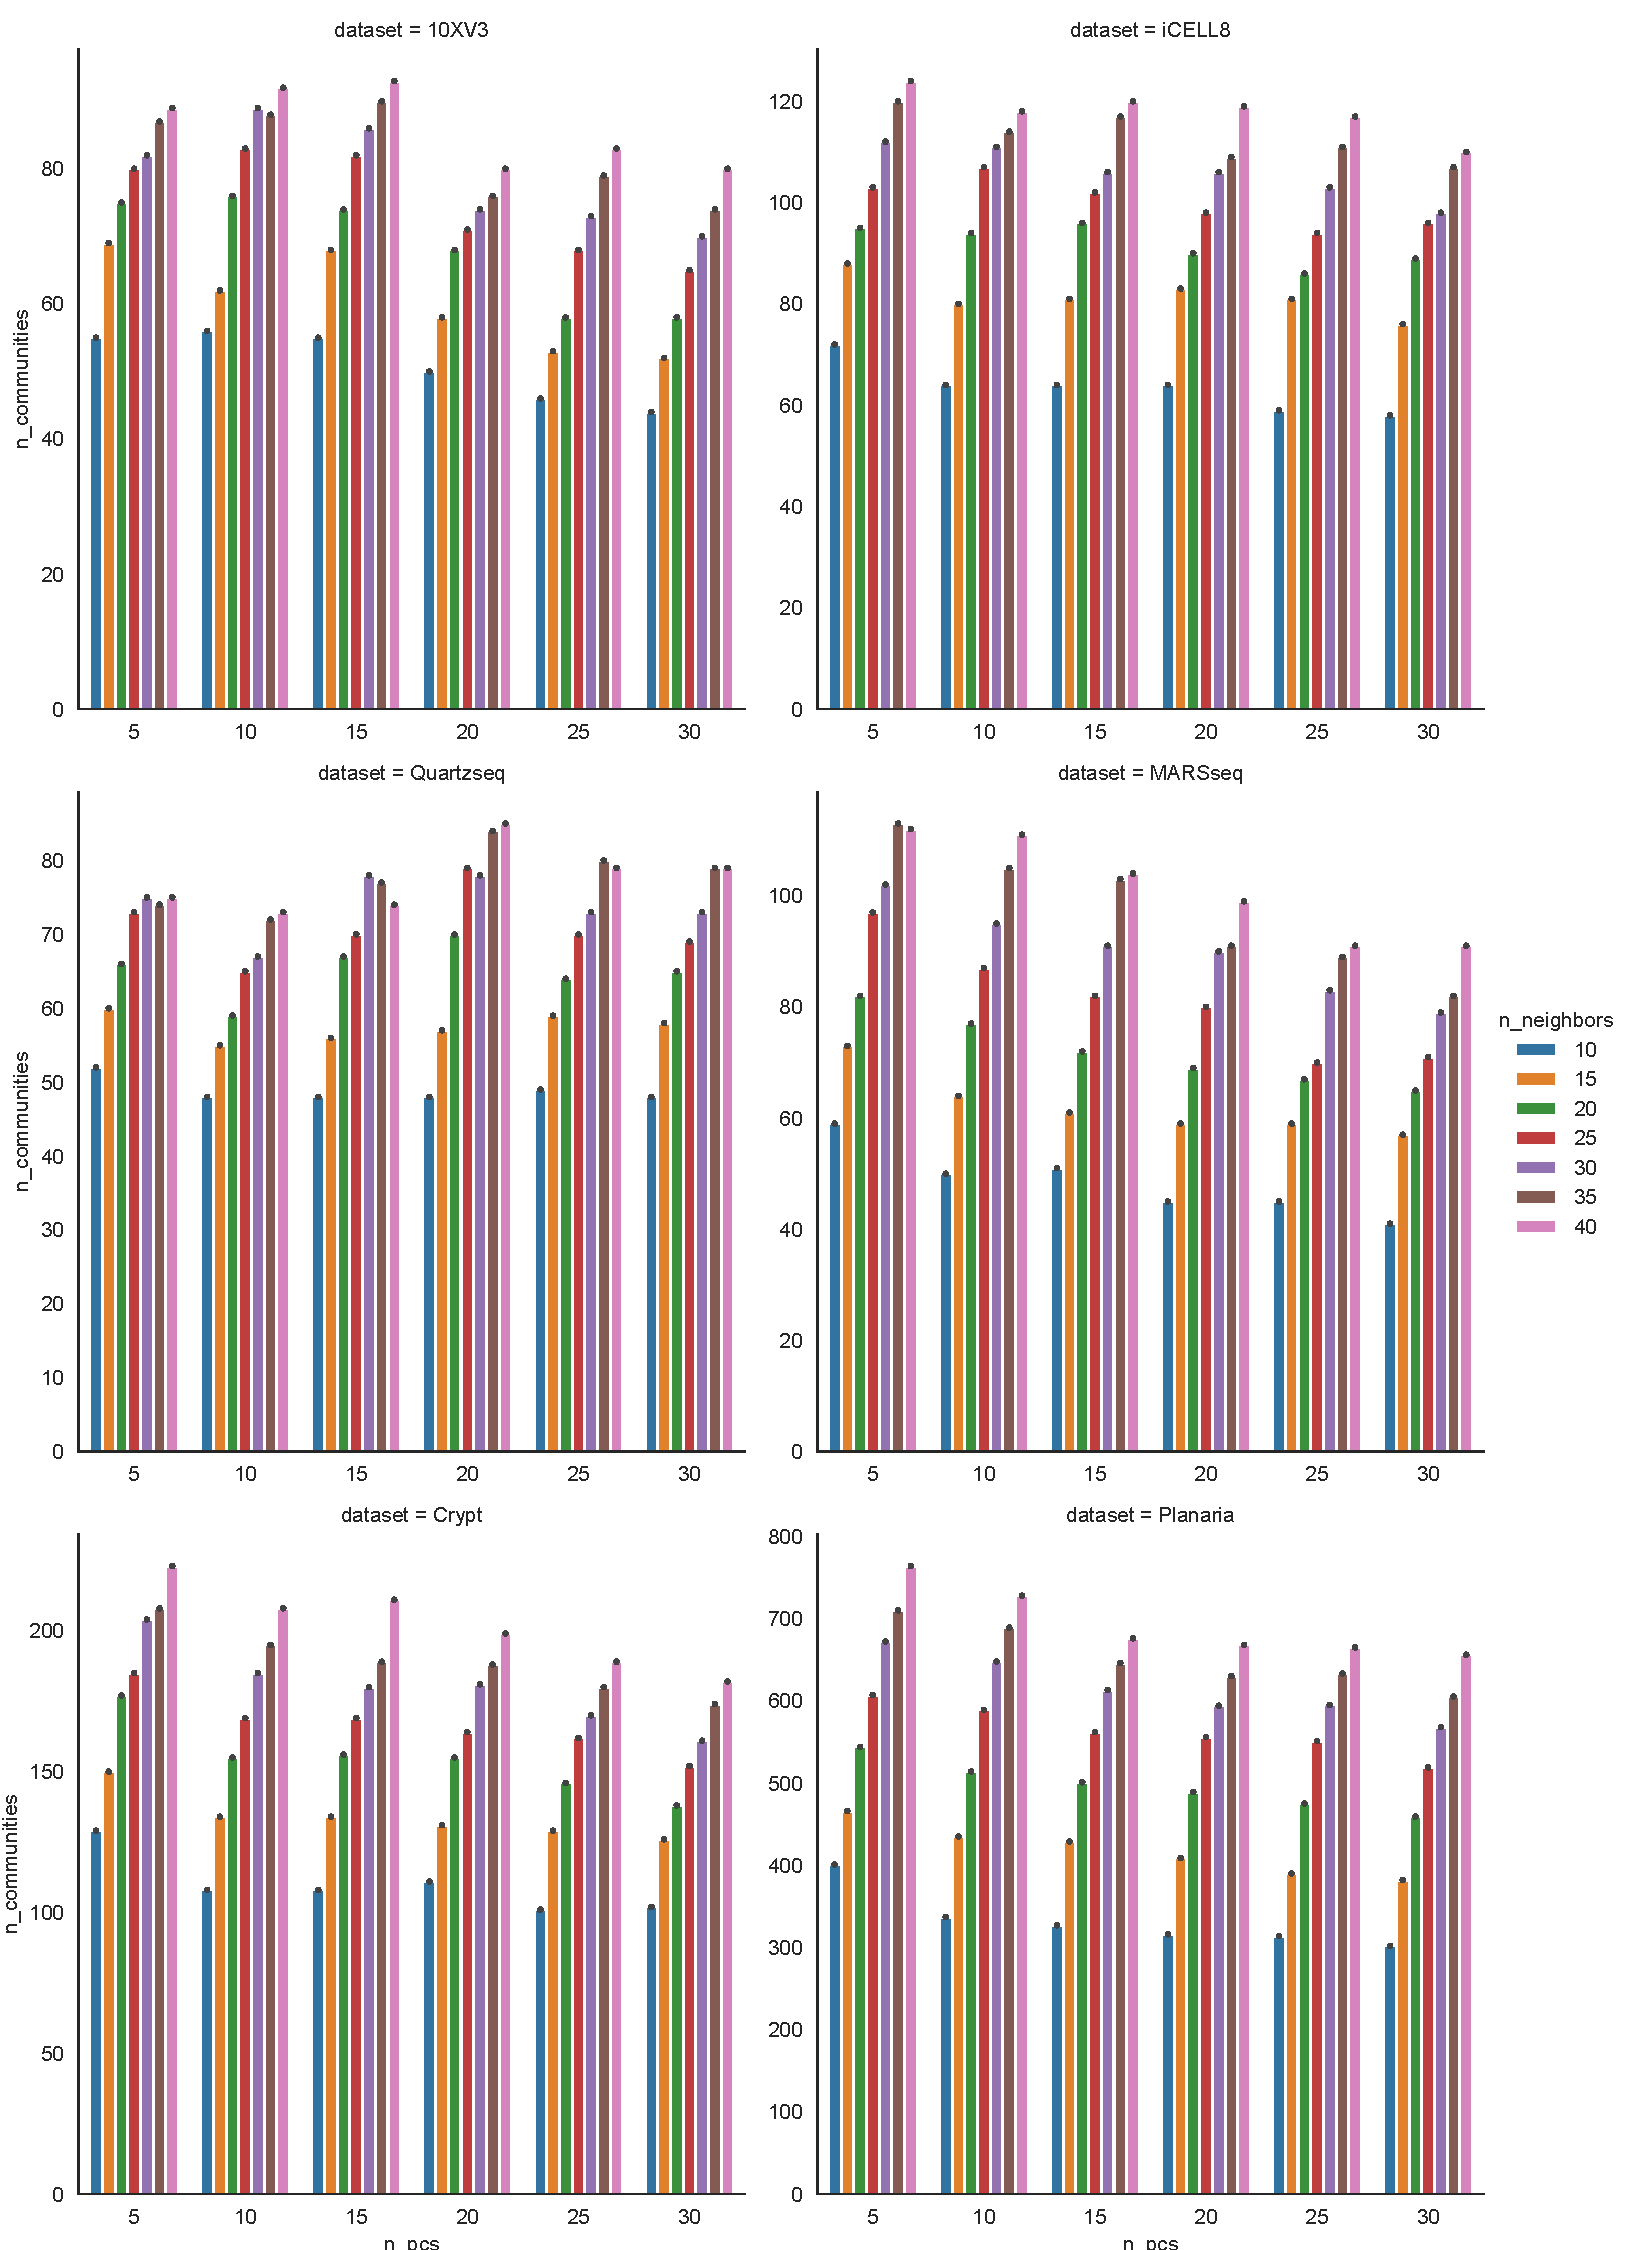
\includegraphics[keepaspectratio,width=.95\textwidth,height=\textheight]{Community_Count_L0.pdf}
%\vspace*{-40pt}
\caption[]{Evaluation of the number of communities. Barplots show the number of communities found at level 0 of the nSBM hierarchy for various datasets used in the manuscript when different parameters are chosen to build the \emph{k}NN graph. Increasing the number of neighbors results in more granular partitioning (\emph{i.e.} more communities), whereas increasing the number of principal components used to evaluate cell-to-cell distance generally works in opposite way. $x$-axis: number of principal components; $y$-axis: number of communities; bar color: number of \emph{k}NN neighbors.} \label{Figure_Comm_Count}
\end{figure}

\clearpage
\begin{figure}[H]
\centering
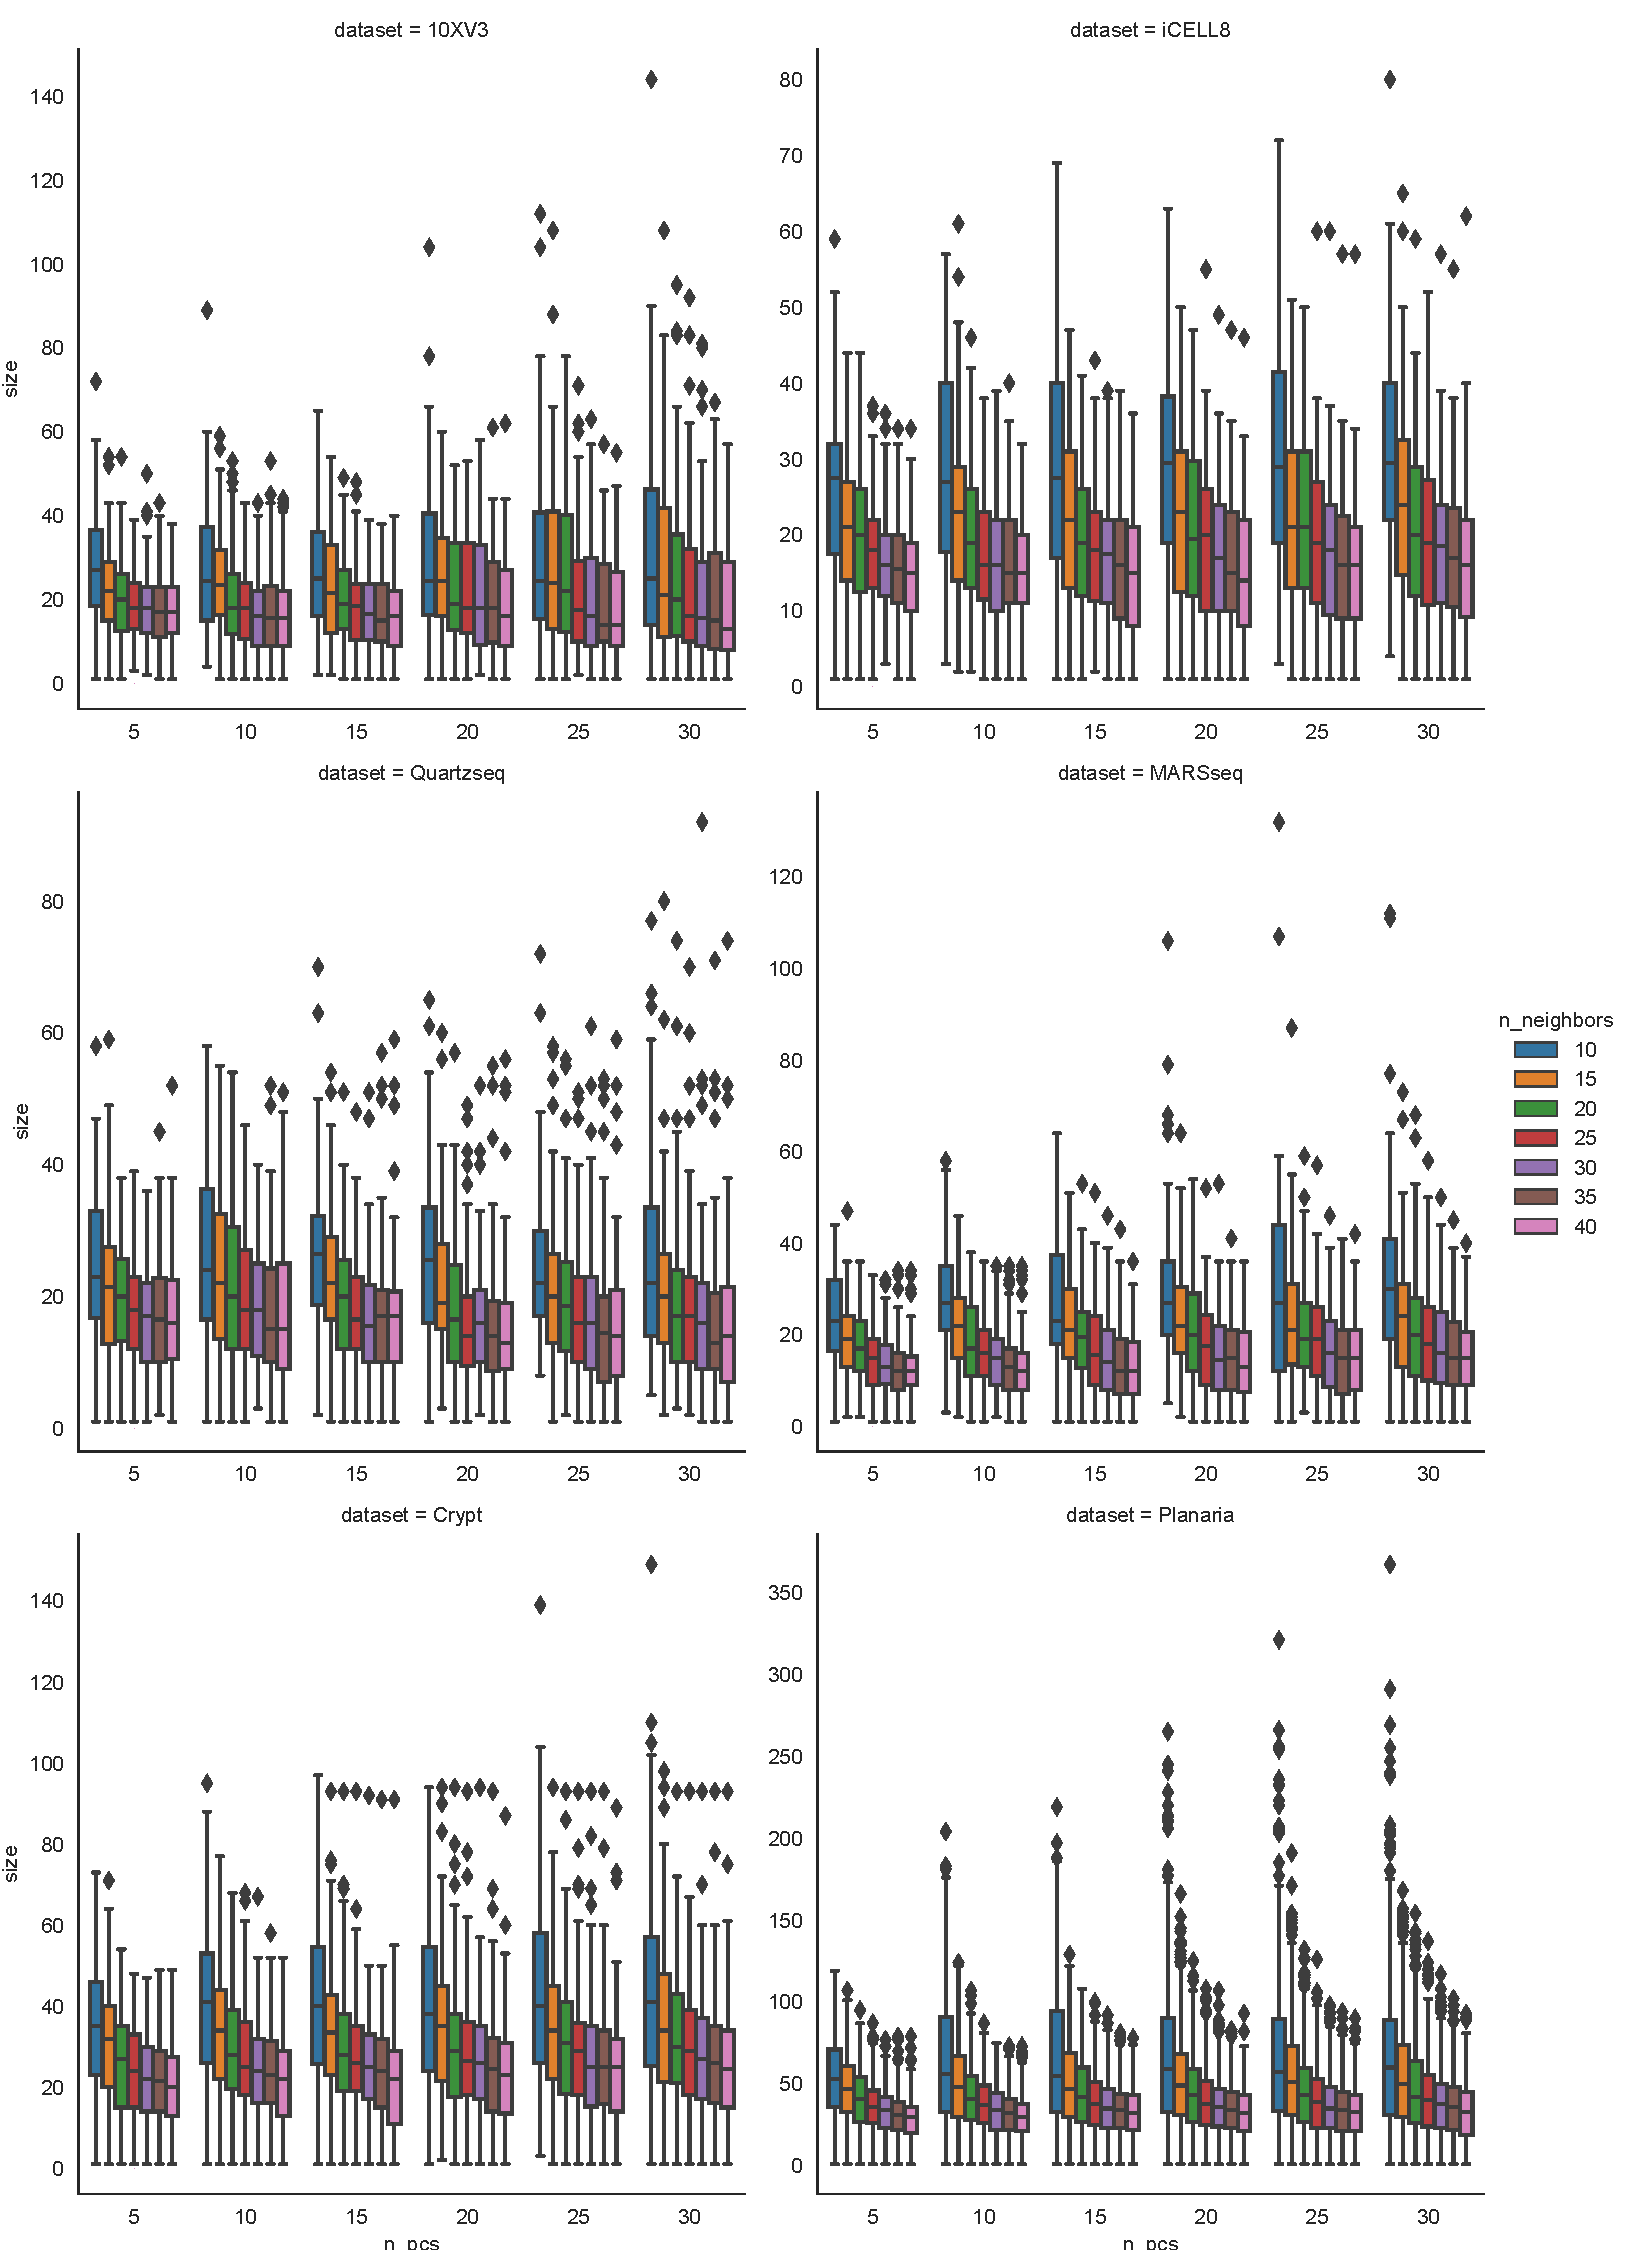
\includegraphics[keepaspectratio,width=.95\textwidth,height=\textheight]{Community_Size_L0.pdf}
%\vspace*{-40pt}
\caption[]{Evaluation of the size of communities. Boxplots show the distribution of size of communities found at level 0 of the nSBM hierarchy for various datasets used in the manuscript when different parameters are chosen to build the \emph{k}NN graph. Increasing the number of neighbors results in more granular partitioning (\emph{i.e.} smaller communities), increasing the number of principal components results in more dispersed sizes. $x$-axis: number of principal components; $y$-axis: community size; bar color: number of \emph{k}NN neighbors.} \label{Figure_Comm_Size}
\end{figure}


\clearpage
\begin{figure}[H]
\centering
    \begin{subfigure}[t]{0.3\textwidth}
        \centering
        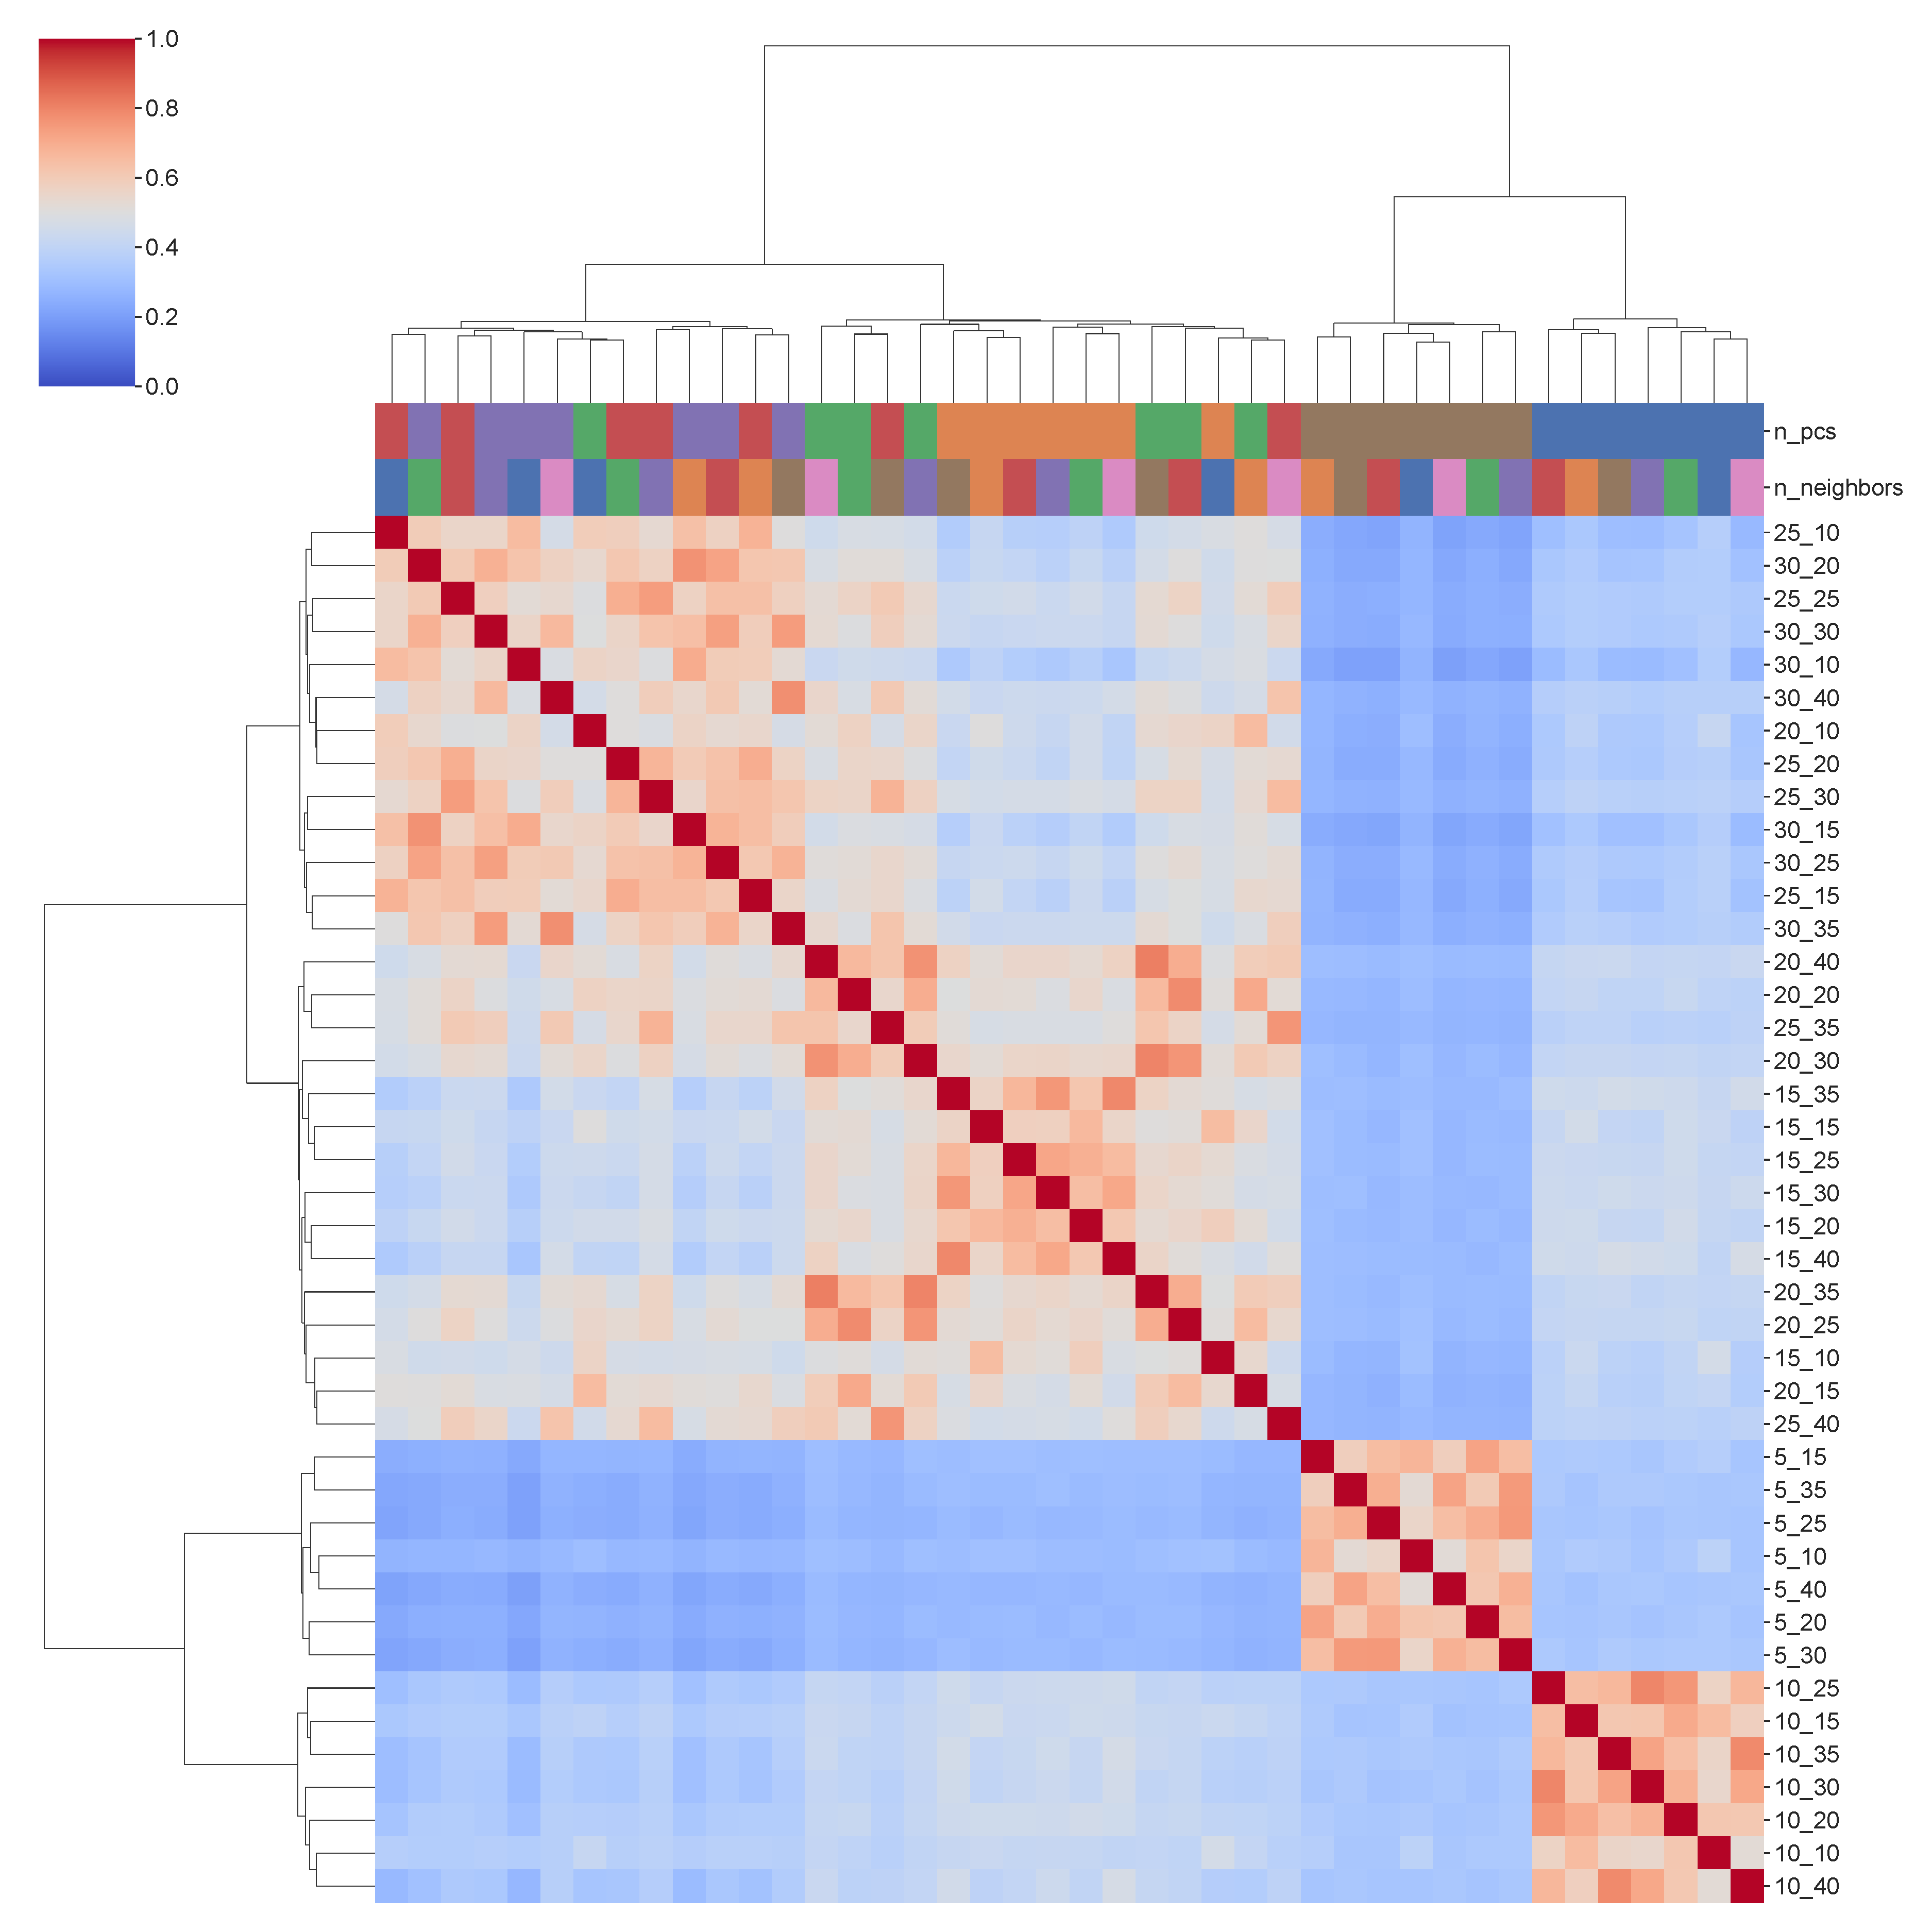
\includegraphics[width=\textwidth]{ClusterMap_L0_Panel0.pdf} 
        \caption{Chromium 10x} \label{cm_10x}
    \end{subfigure}
    \hfill
    \begin{subfigure}[t]{0.3\textwidth}
        \centering
        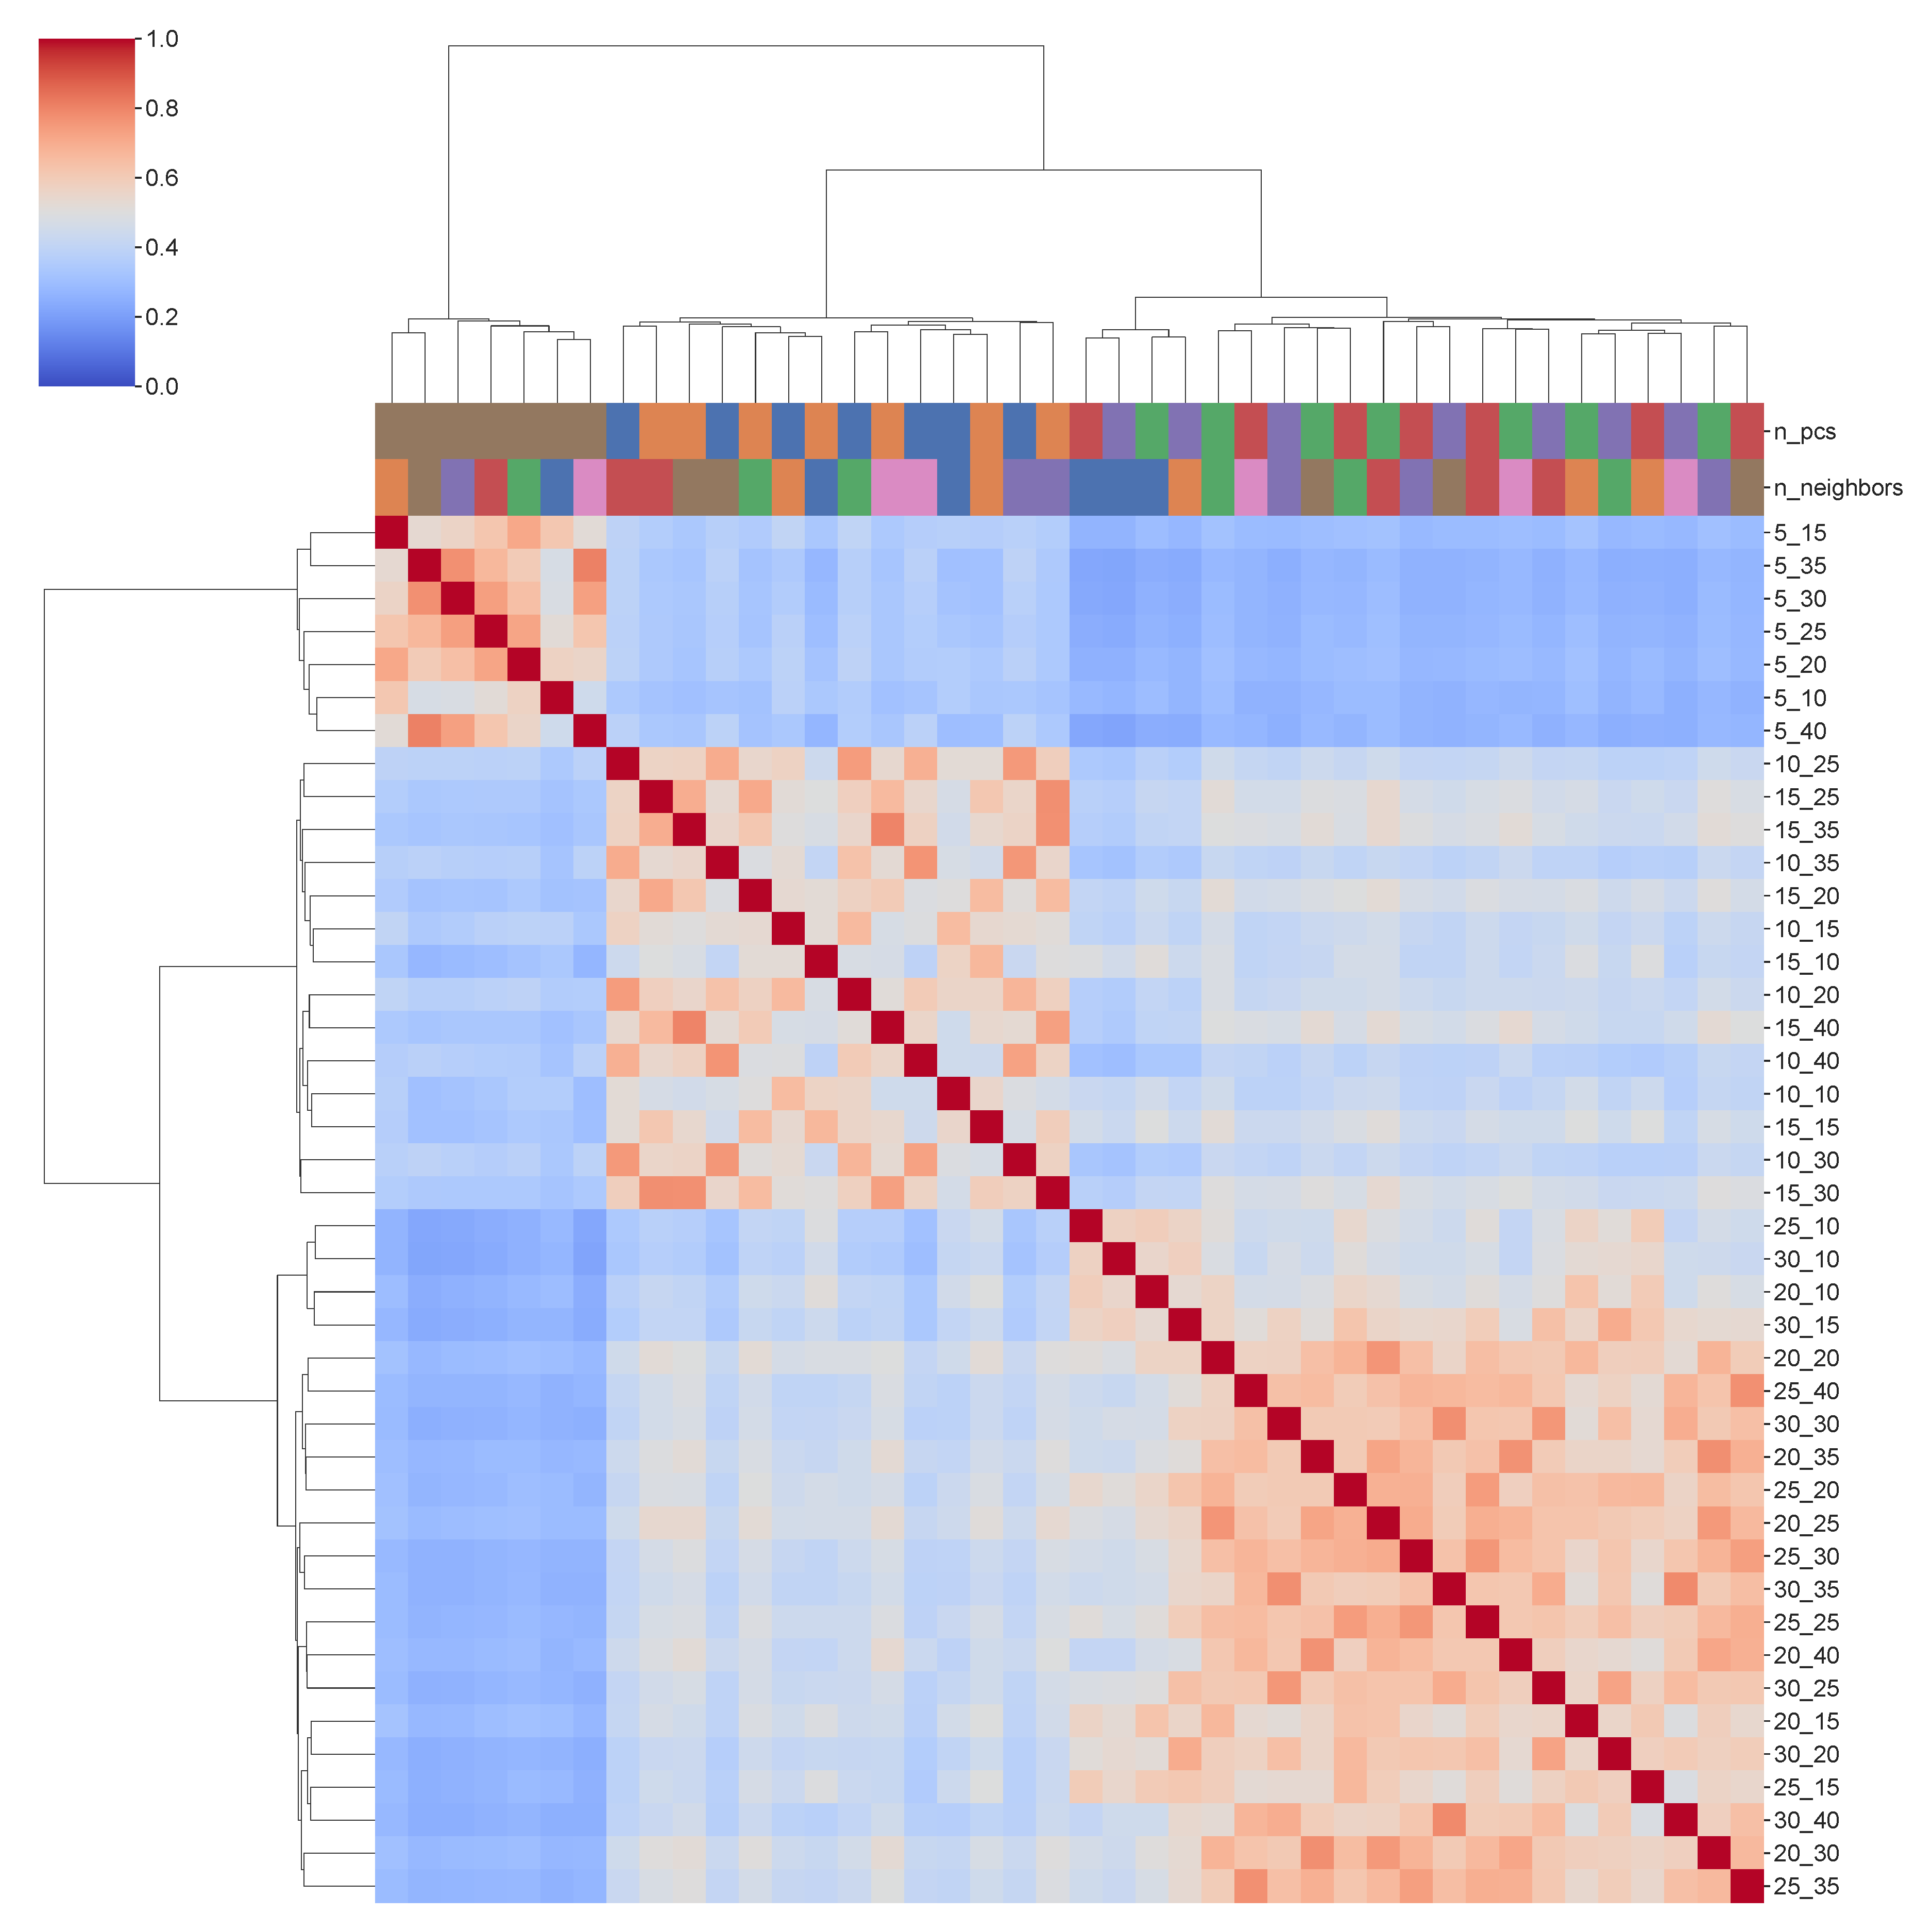
\includegraphics[width=\textwidth]{ClusterMap_L0_Panel1.pdf} 
        \caption{iCell8} \label{cm_icell8}
    \end{subfigure}
    \hfill
%    \vspace{40pt}
    \begin{subfigure}[t]{0.3\textwidth}
        \centering
        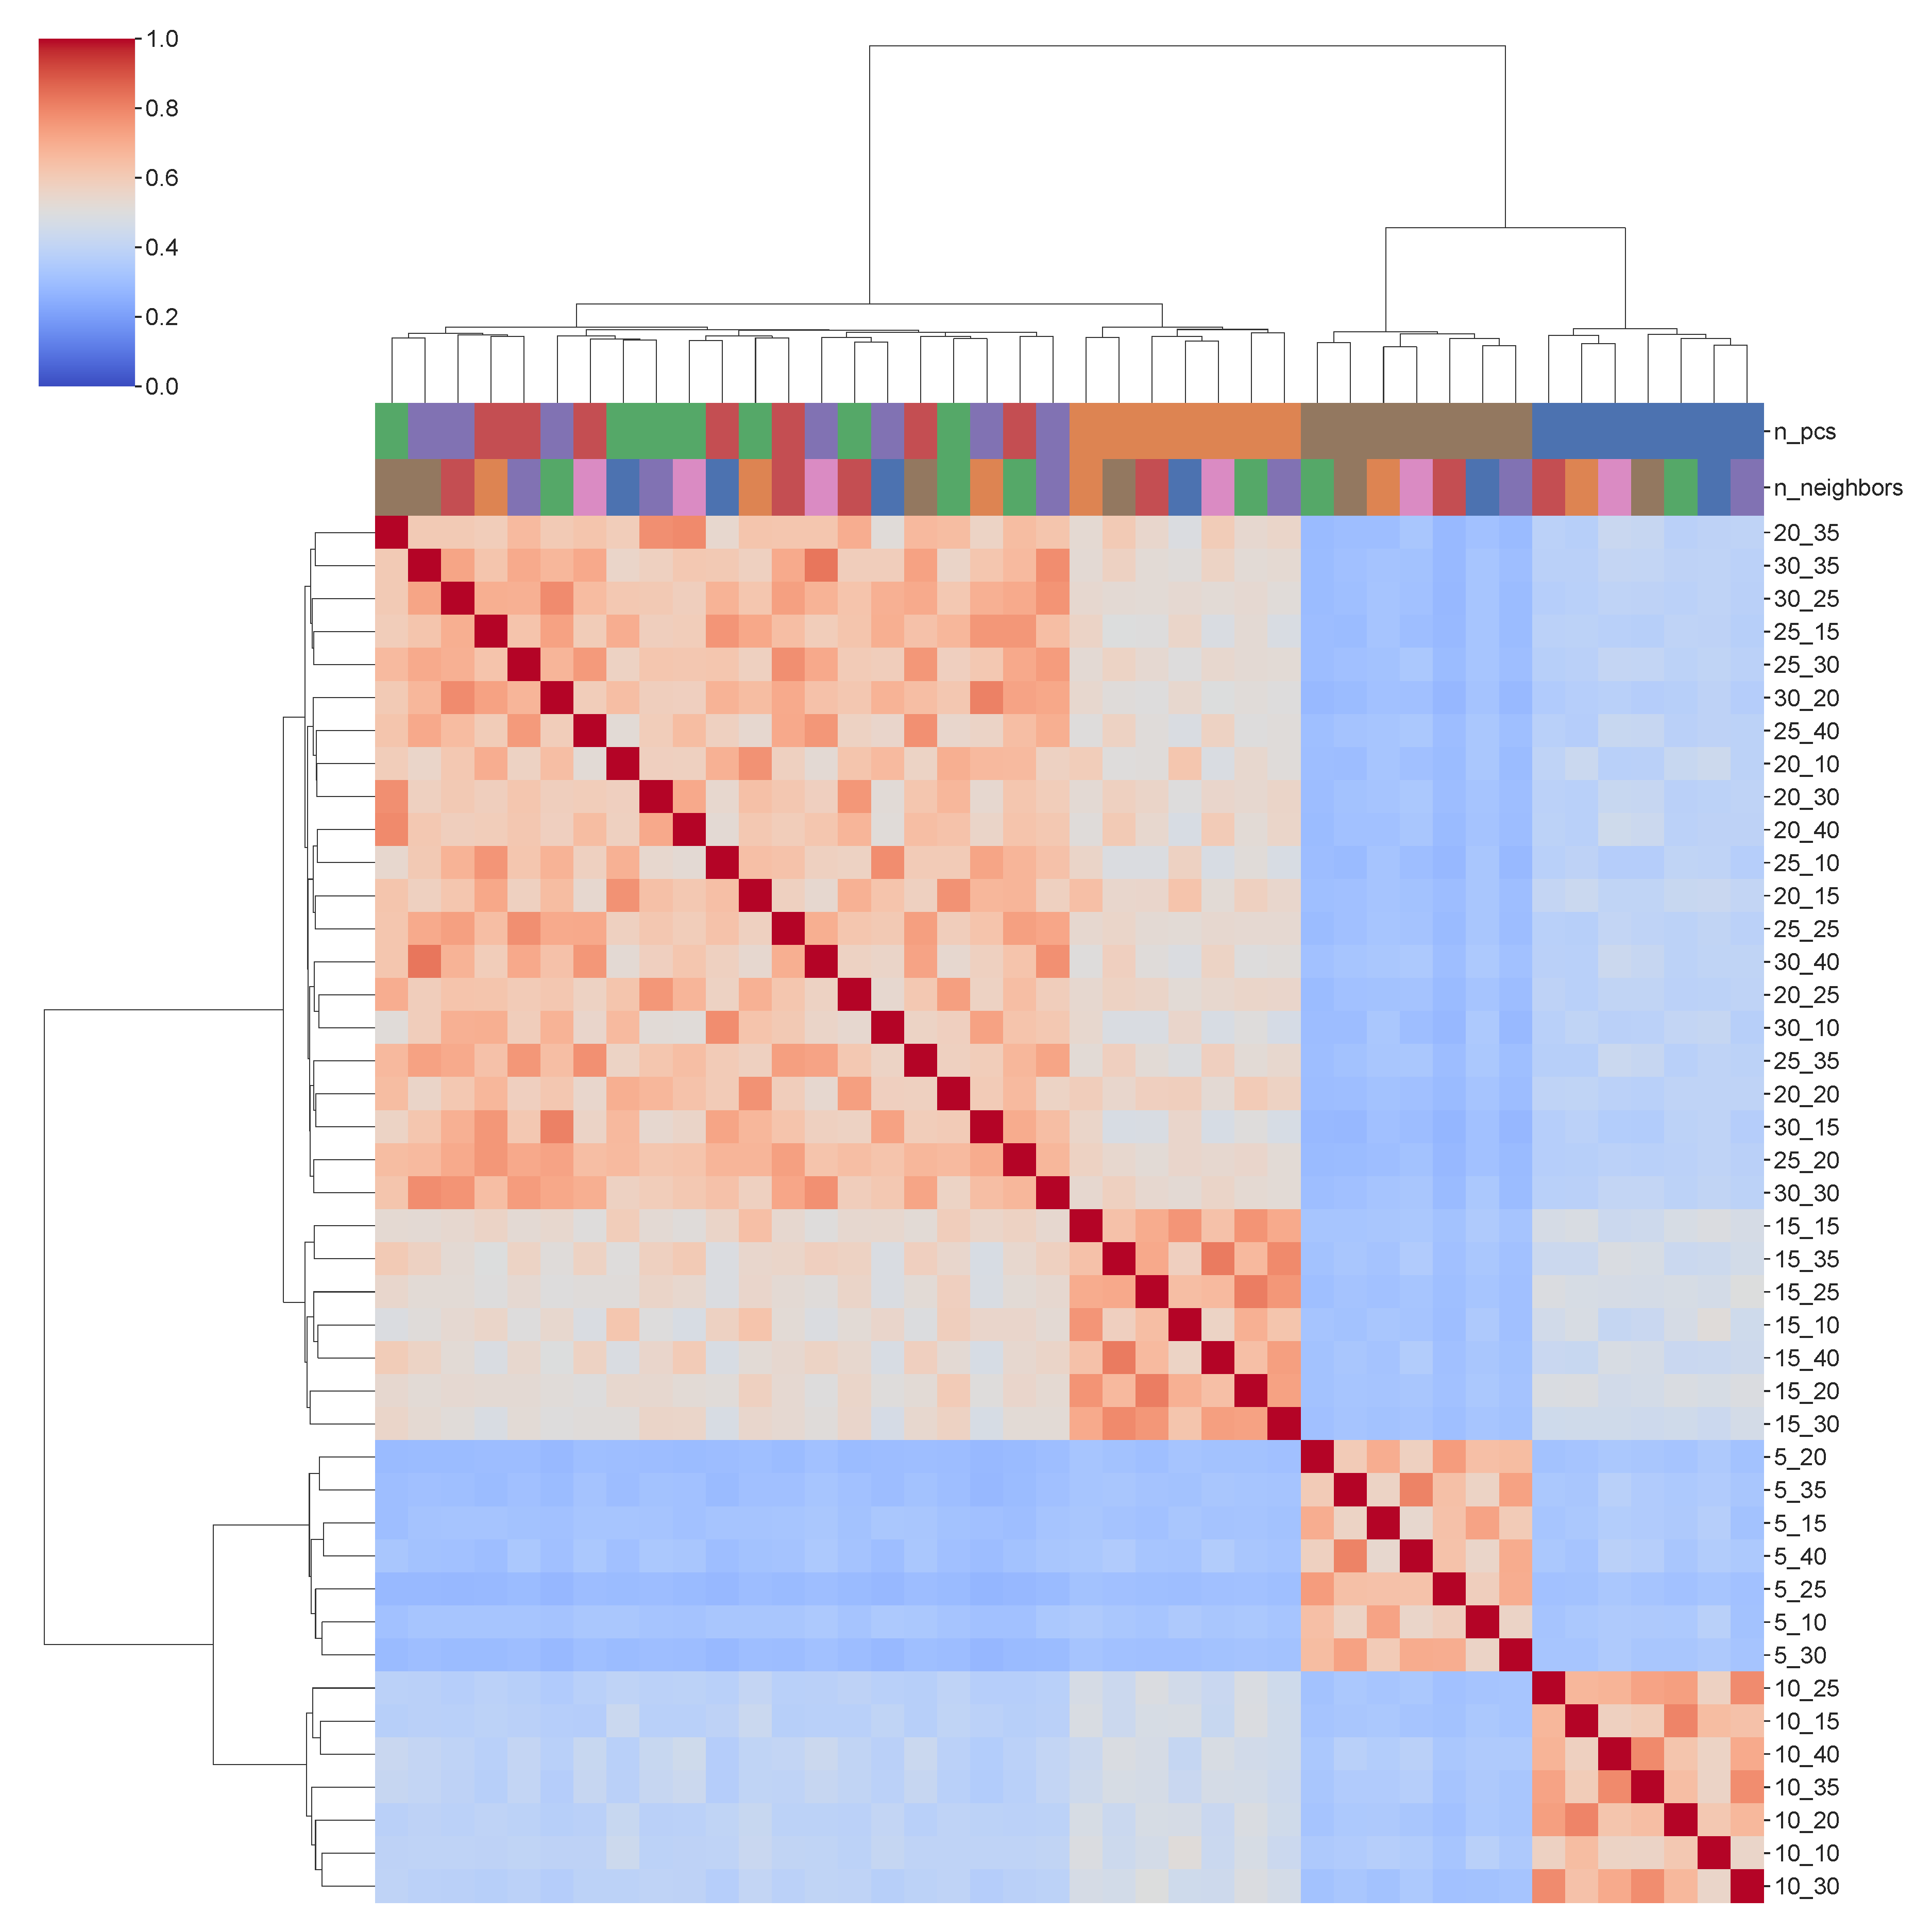
\includegraphics[width=\textwidth]{ClusterMap_L0_Panel2.pdf} 
        \caption{Quartz-seq2} \label{cm_quartz}
    \end{subfigure}

    \begin{subfigure}[t]{0.3\textwidth}
        \centering
        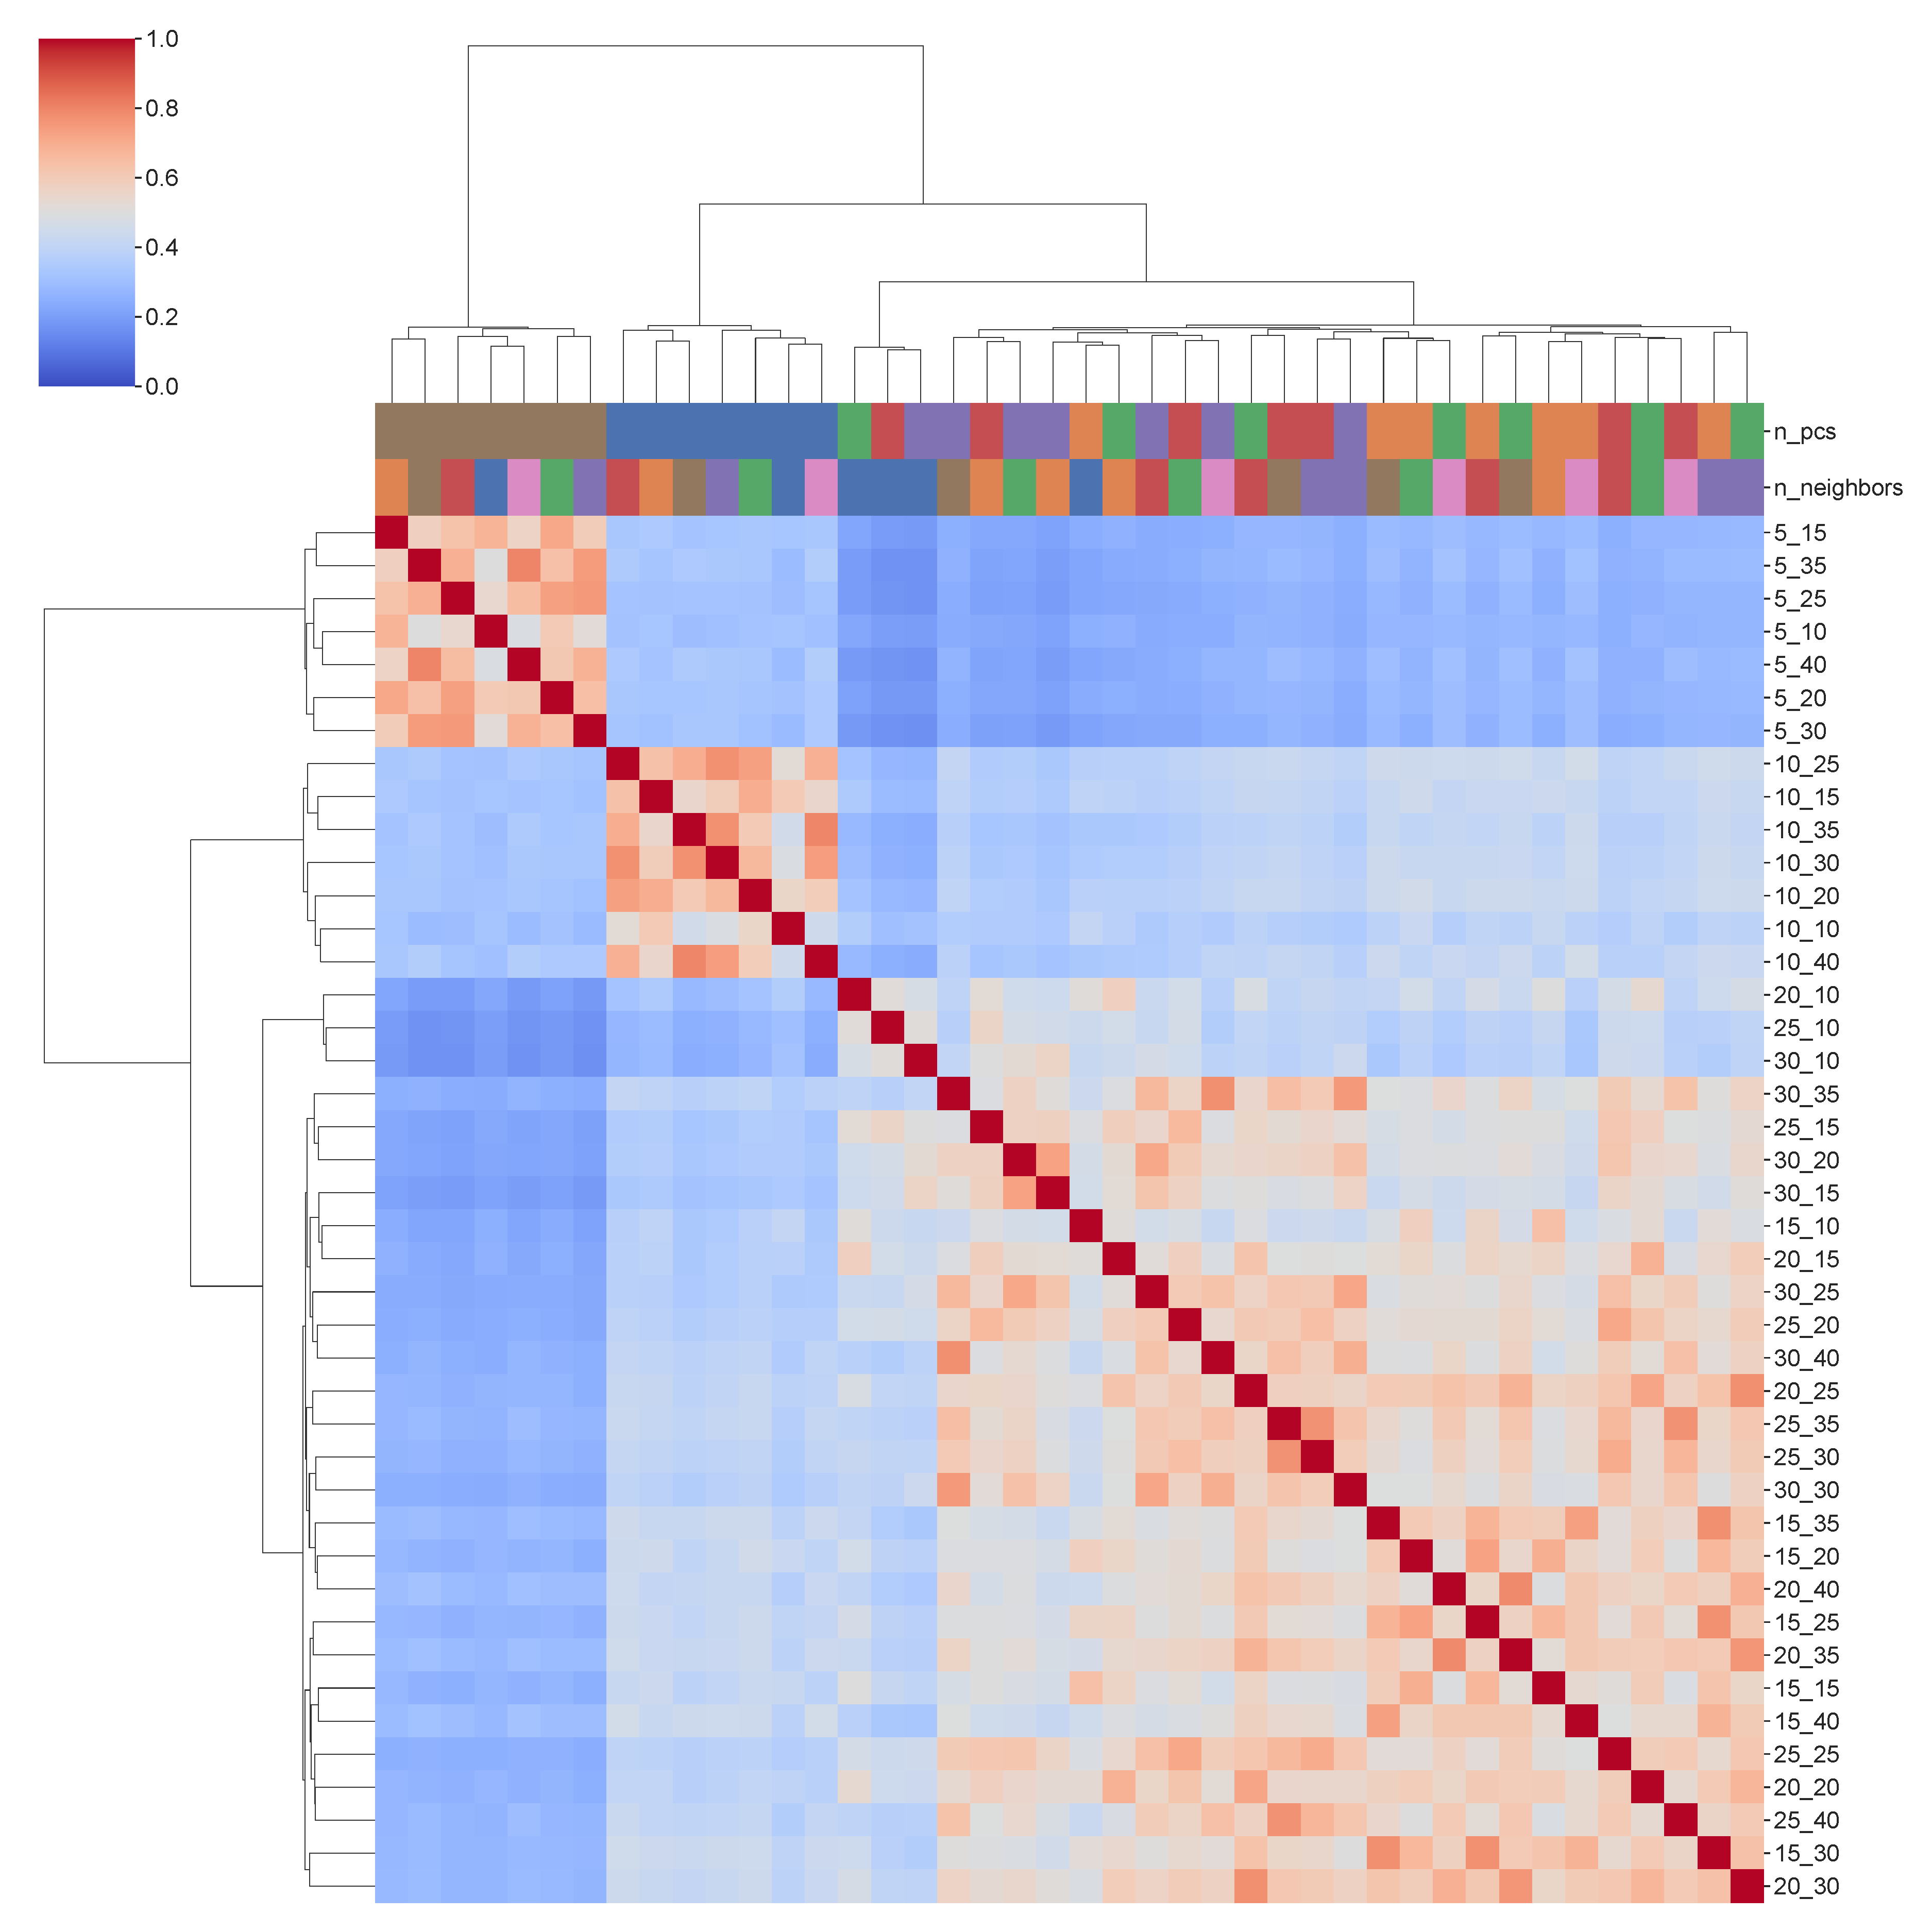
\includegraphics[width=\textwidth]{ClusterMap_L0_Panel3.pdf} 
        \caption{MARS-seq} \label{cm_mars}
    \end{subfigure}
%    \vspace{40pt}
   \hfill
    \begin{subfigure}[t]{0.3\textwidth}
        \centering
        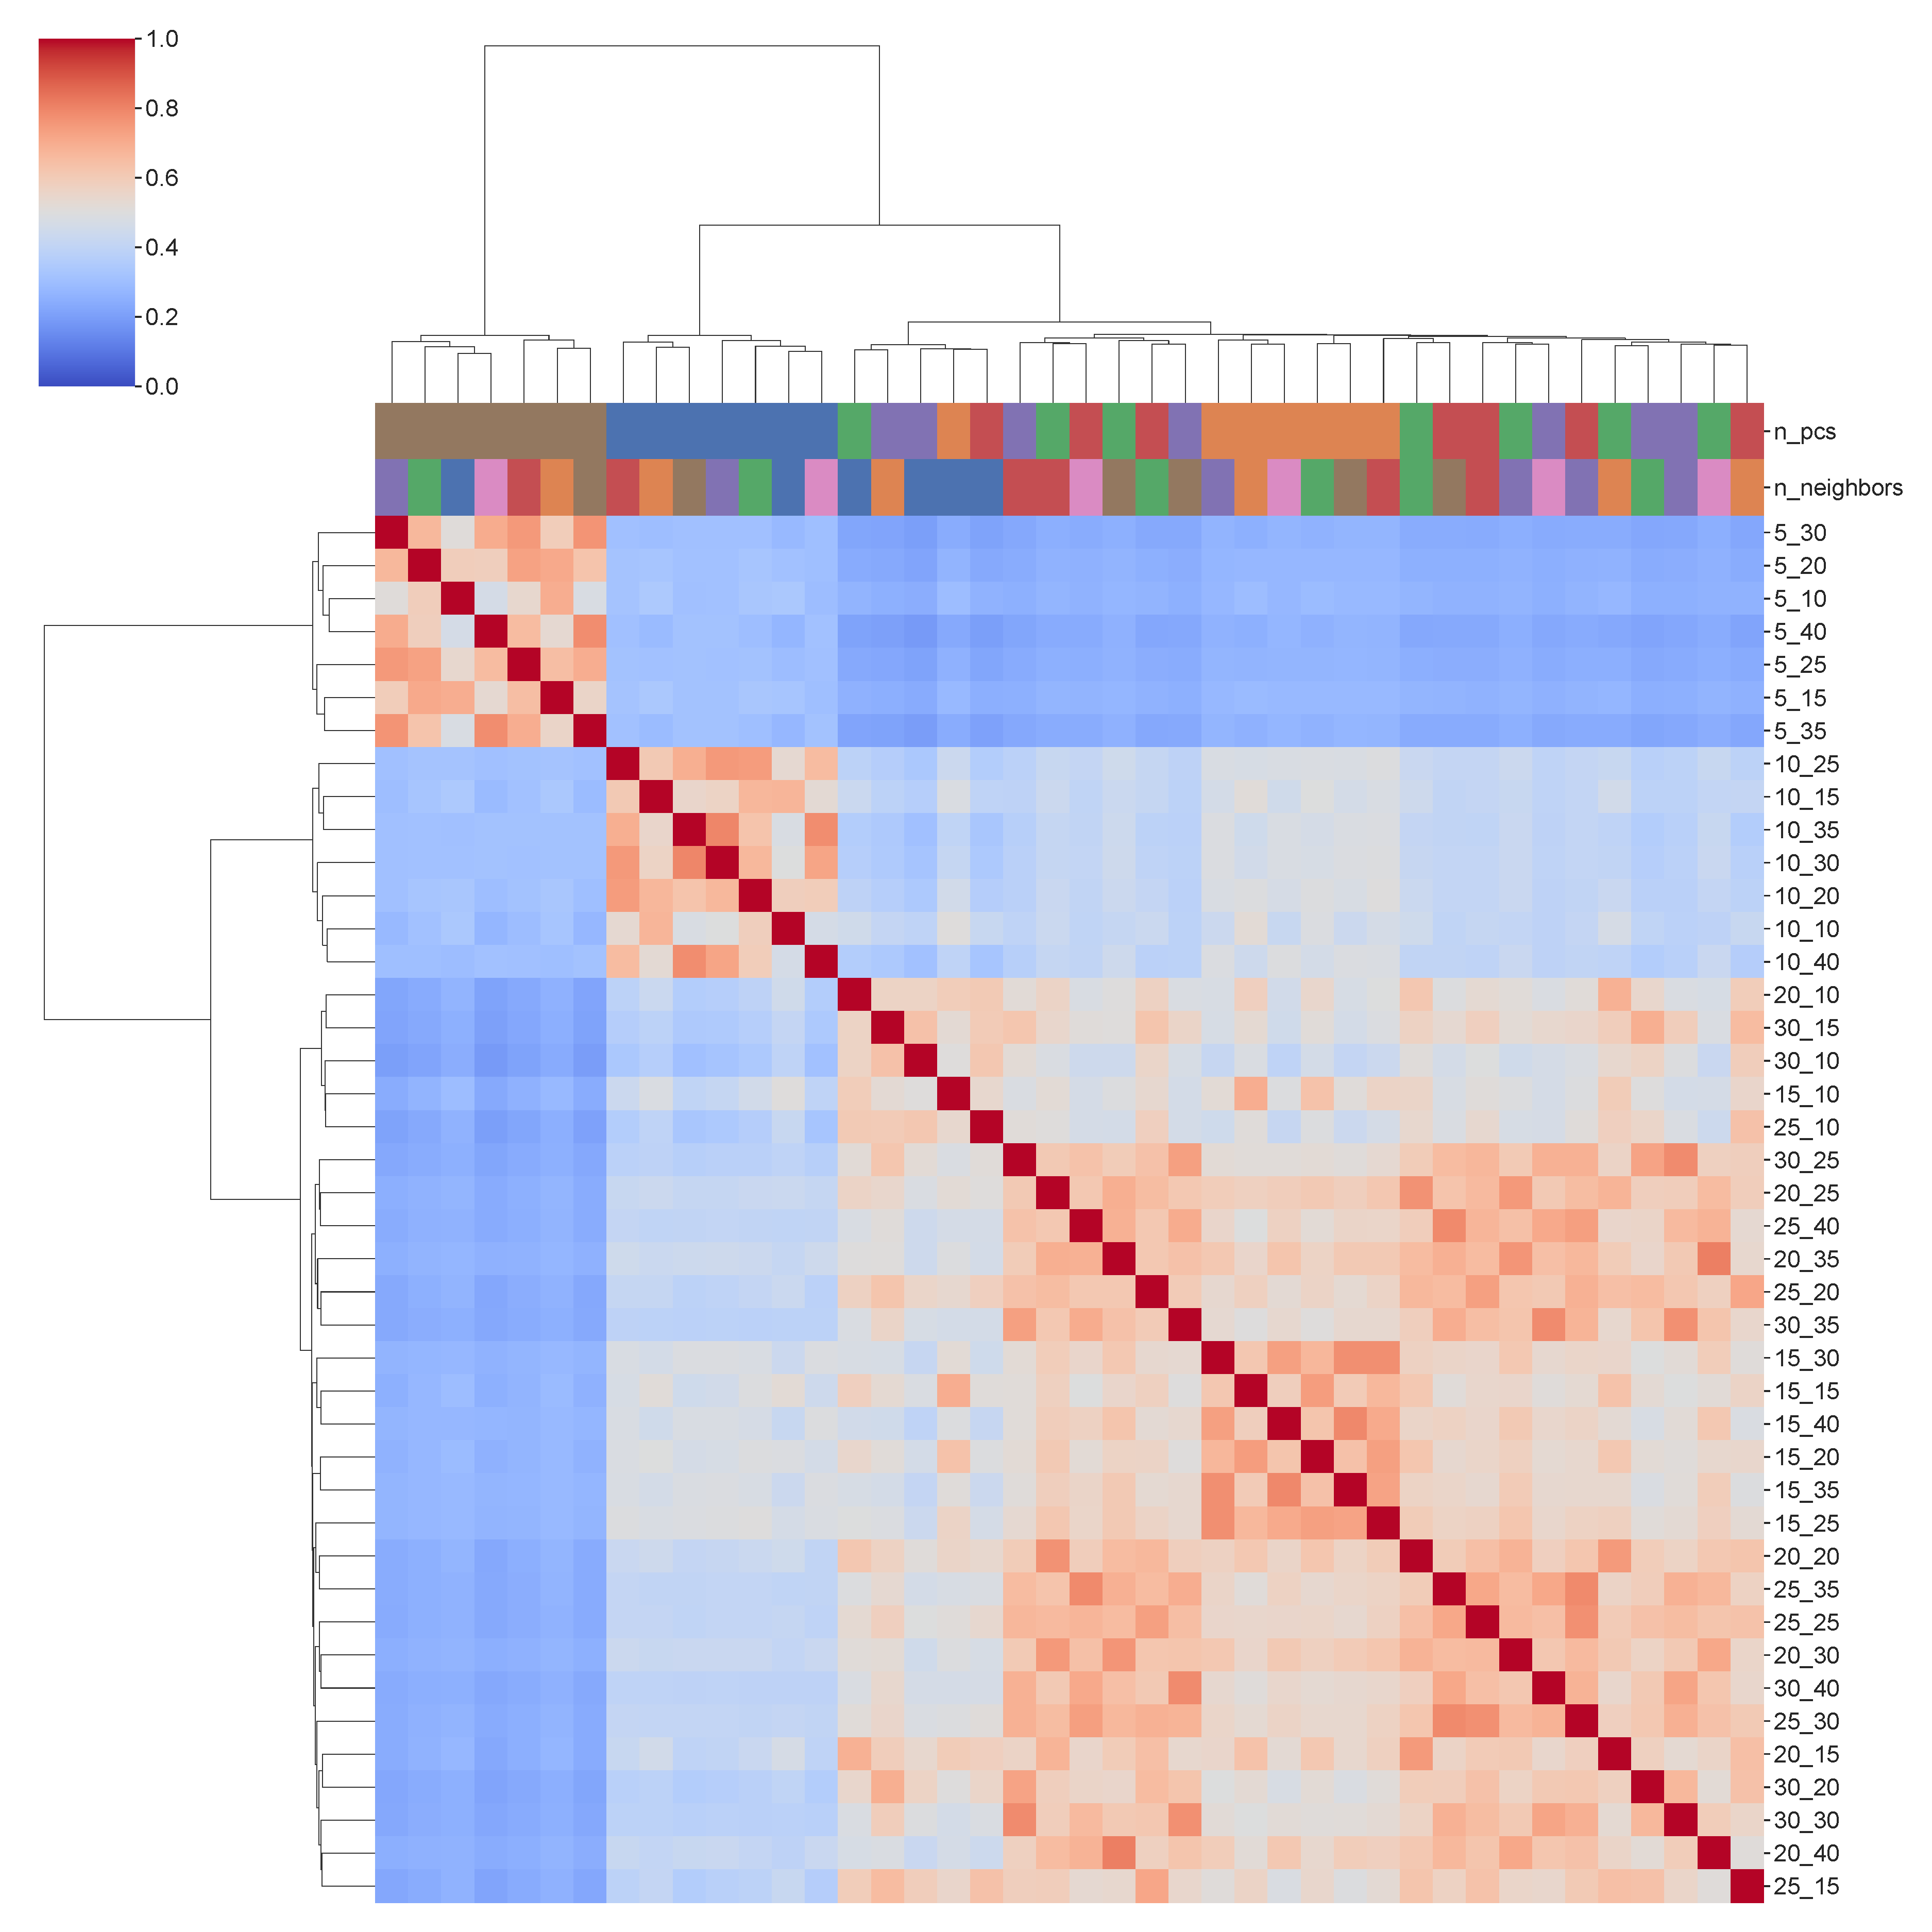
\includegraphics[width=\textwidth]{ClusterMap_L0_Panel4.pdf} 
        \caption{Crypt cells} \label{cm_crypt}
    \end{subfigure}
    \hfill
    \begin{subfigure}[t]{0.3\textwidth}
        \centering
        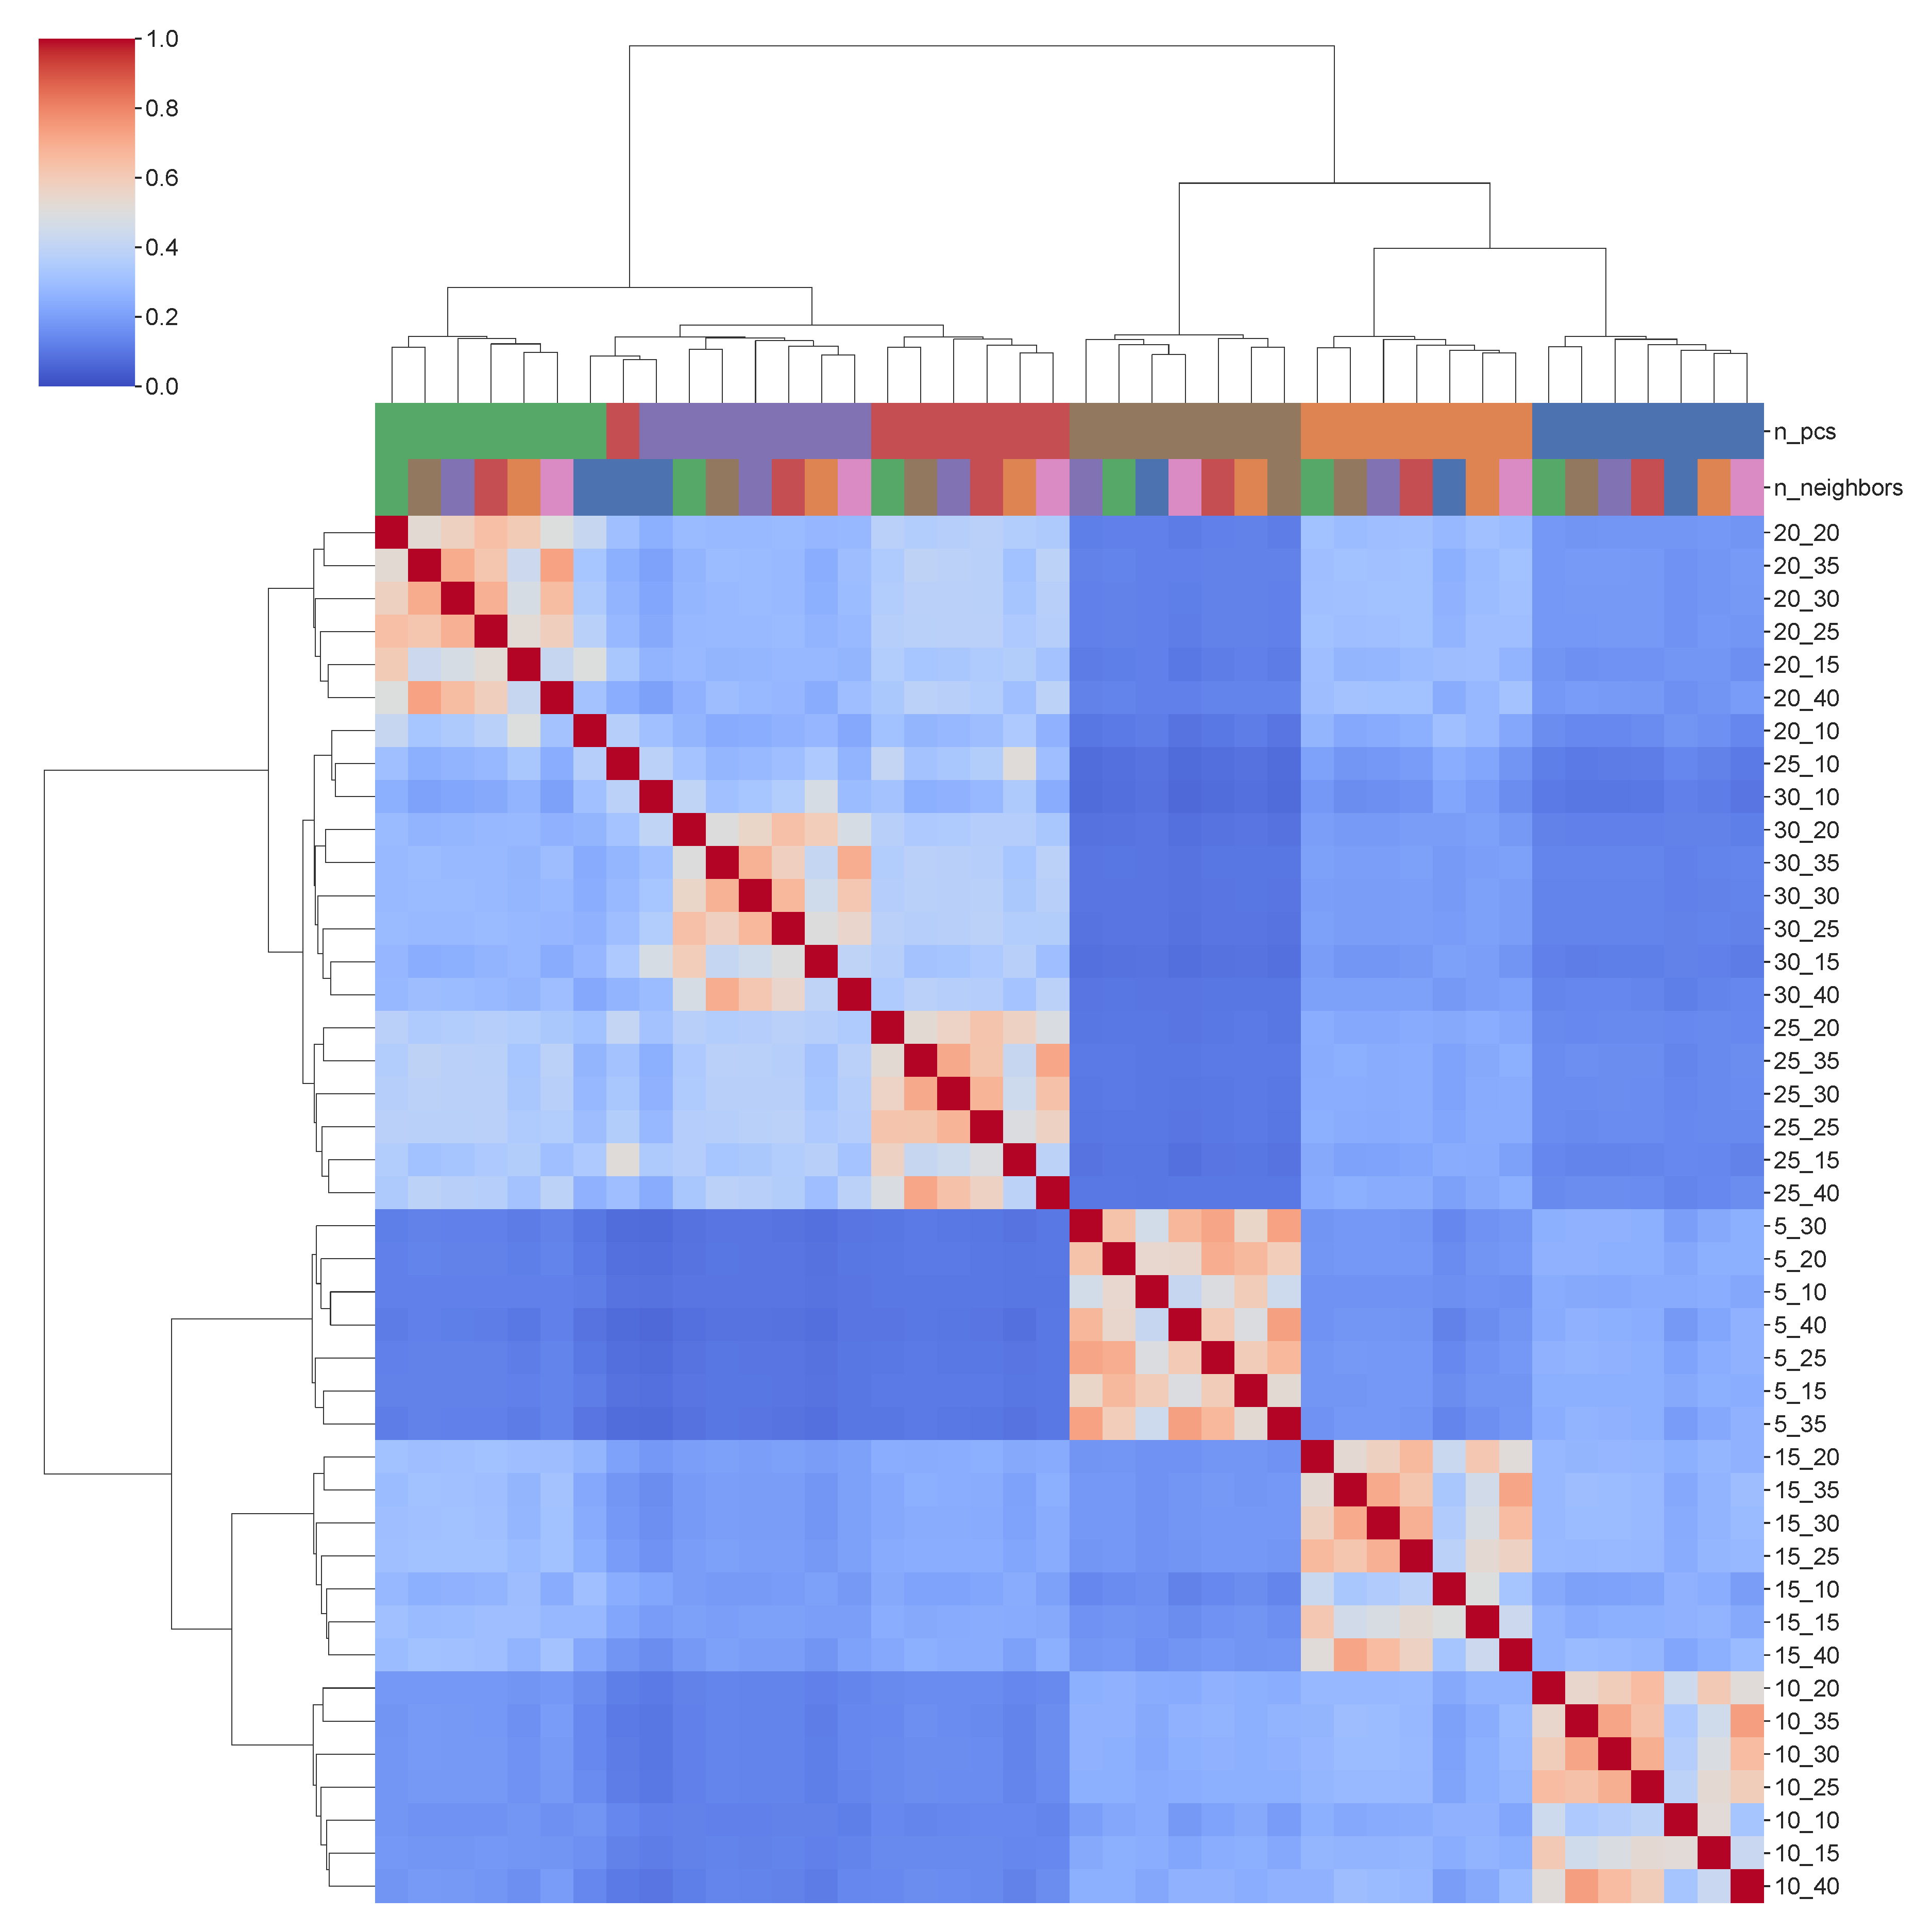
\includegraphics[width=\textwidth]{ClusterMap_L0_Panel5.pdf} 
        \caption{Planaria} \label{cm_planaria}
    \end{subfigure}
    \vspace{40pt}


%\vspace*{-40pt}
\caption[]{Consistency at Level 0. Each heatmap shows the Adjusted Rand Index among partitions found when different parameters are used to build th \emph{k}NN graph. Row labels encode the number of PCs and the number of neighbors (P\_N), reflected in colors used to annotate columns.} \label{Figure_Clustermap_L0}
\end{figure}


\end{document}
